%\chapterimage{Pictures/SDG Wheel_PRINT.jpg}
% Chapter heading image
\chapter{Cadre conceptuel et Méthodologie}


\section{Cadre conceptuel}

\subsection{Introduction générale aux ODD}

Les Objectifs de Développement Durable (ODD) ont été adoptés en septembre 2015 par l’Assemblée générale des Nations Unies dans le cadre de l’Agenda 2030. Ils constituent un cadre universel et intégré visant à éradiquer la pauvreté, protéger la planète et garantir la prospérité pour tous, dans le respect du principe fondamental de \textit{``Ne laisser personne de côté''}.  

Succédant aux Objectifs du Millénaire pour le Développement (OMD, 2000–2015), les ODD introduisent une vision élargie et multidimensionnelle du développement durable, couvrant les aspects économiques, sociaux et environnementaux. Ils sont universels, applicables à tous les pays, et interconnectés, soulignant l’importance d’une approche intégrée du développement.  

\subsection{Présentation des 17 ODD}

Les Objectifs de Développement Durable (ODD) se déclinent en 17 objectifs principaux, 169 cibles et plus de 230 indicateurs. 
Le tableau ci-dessous présente les 17 ODD avec leurs intitulés respectifs.  

% Ligne 1
\noindent
\begin{minipage}[t]{0.48\textwidth}
	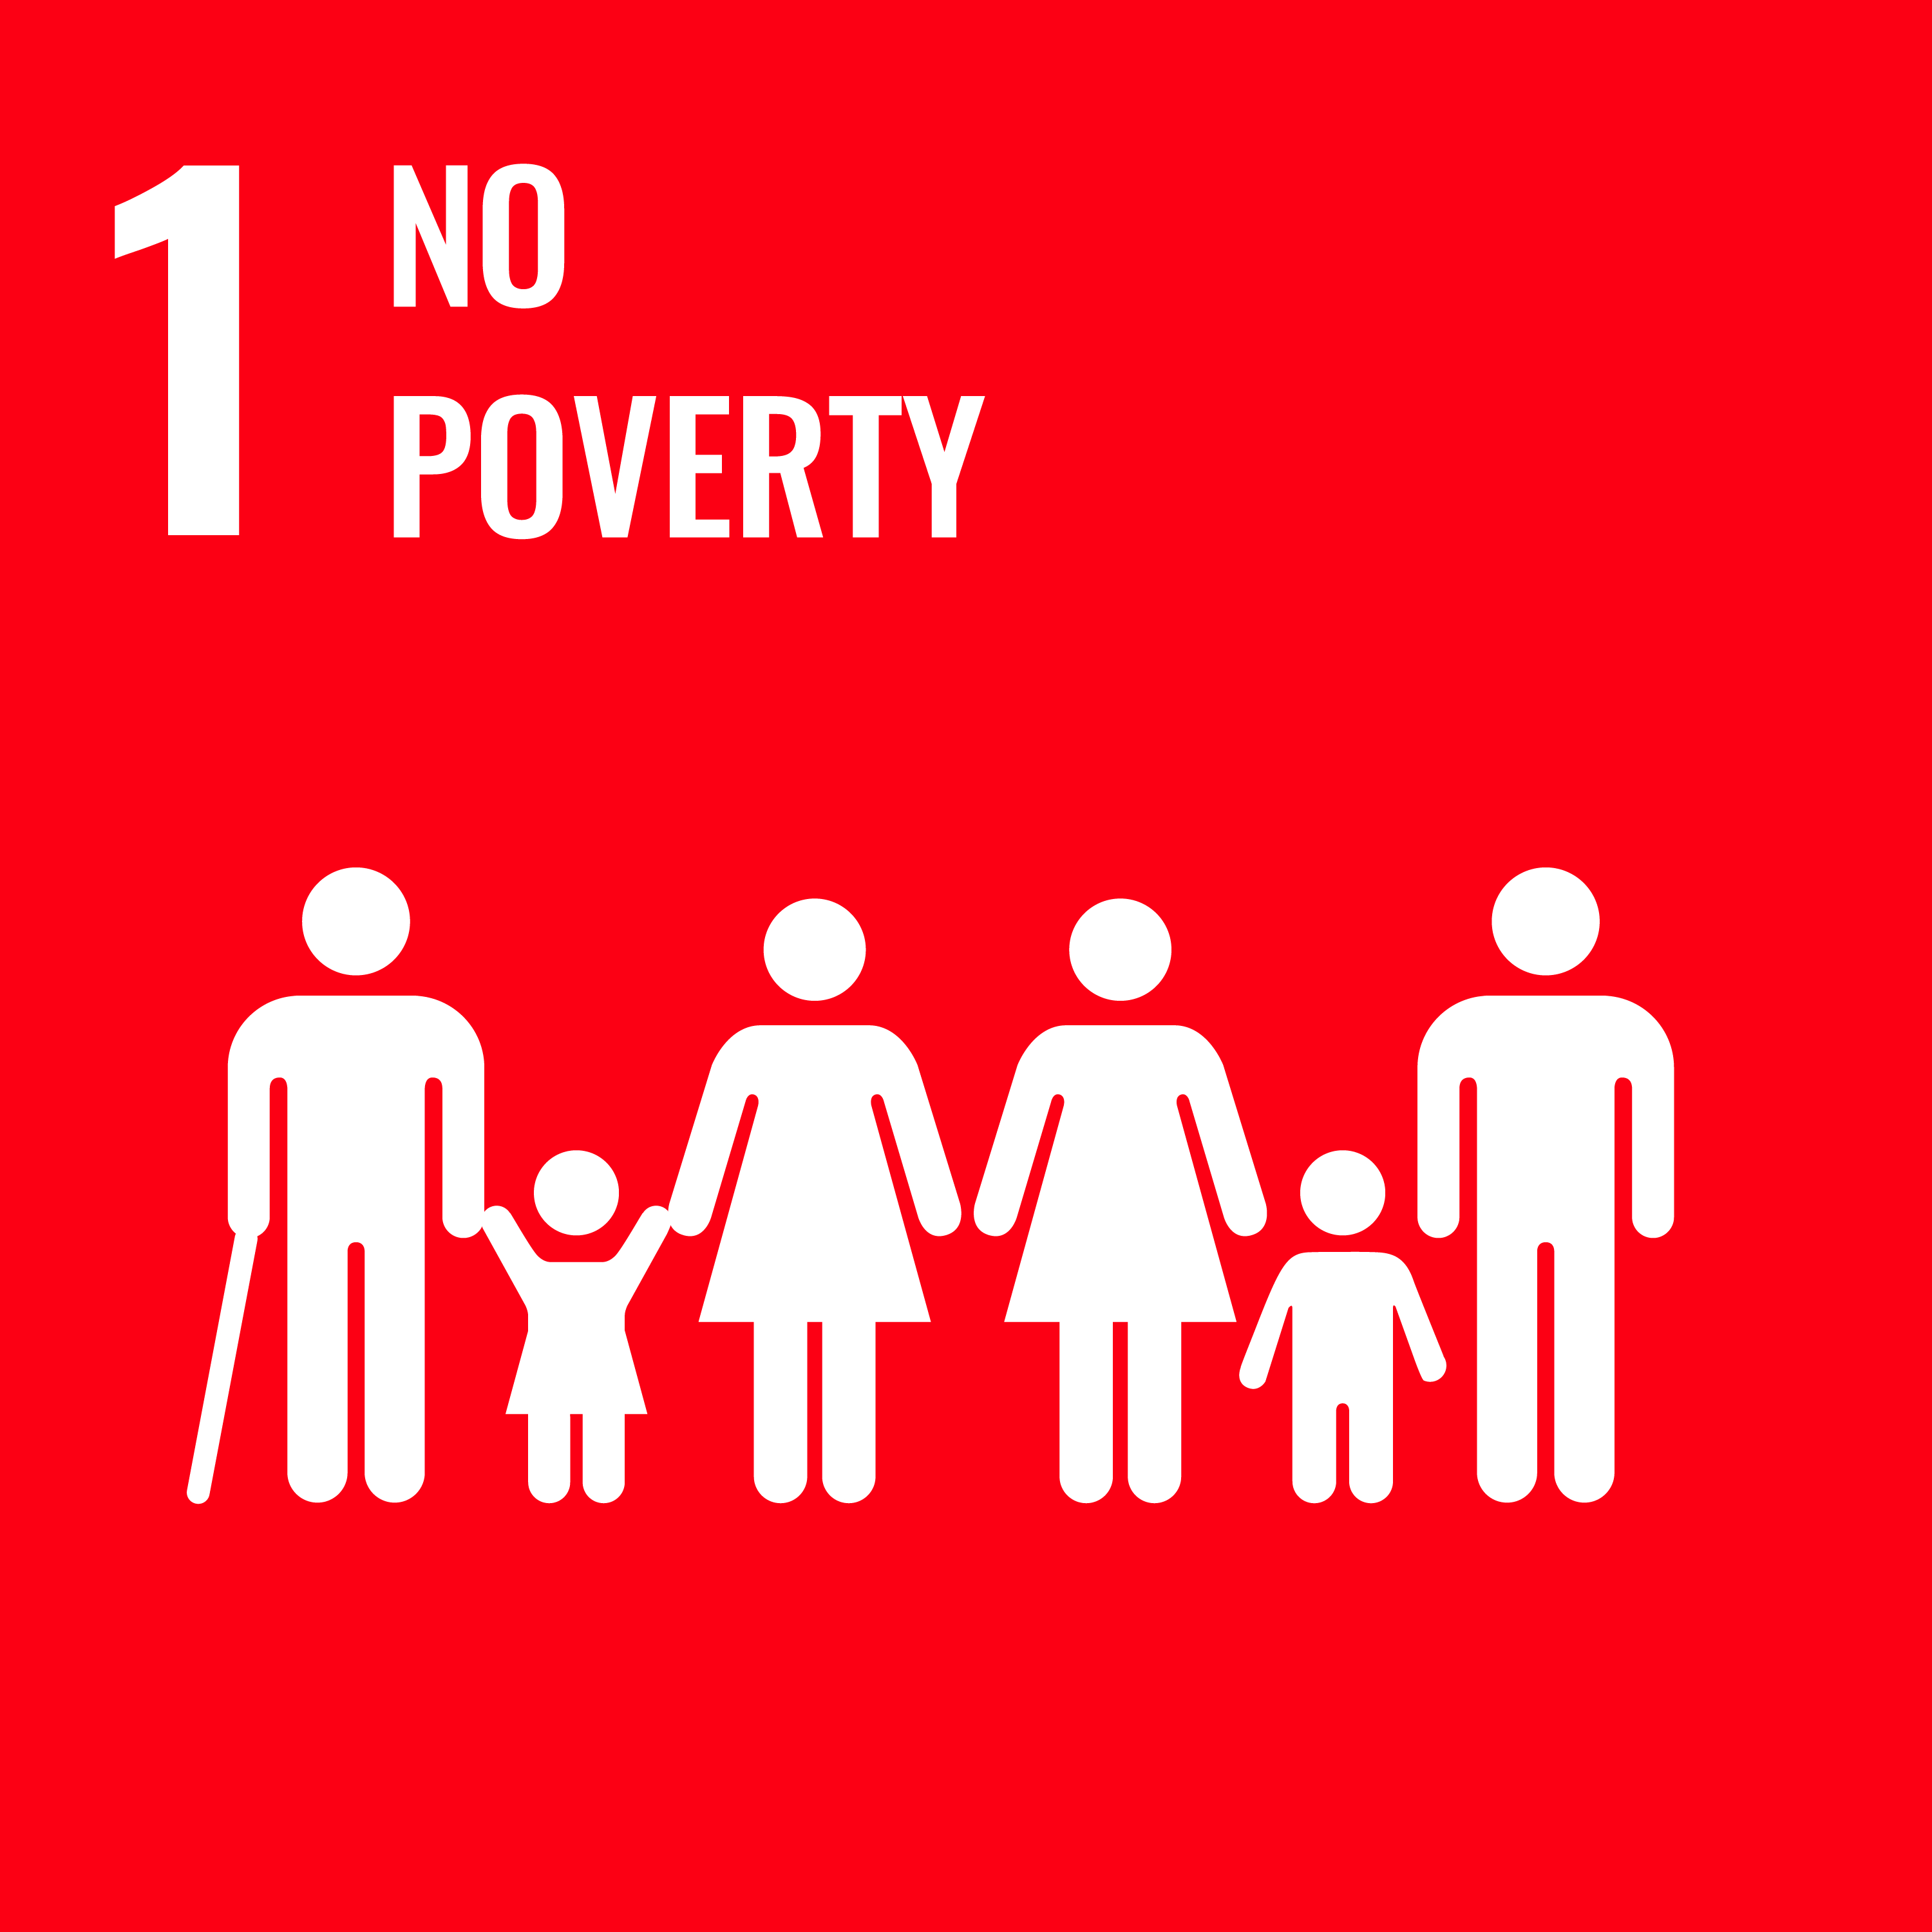
\includegraphics[width=0.25\linewidth]{Pictures/ODD/ODD01.jpg}%
	\hspace{0.5em}%
	\parbox[t]{0.7\linewidth}{\textbf{ODD 1 : Pas de pauvreté} -- Mettre fin à la pauvreté sous toutes ses formes et partout dans le monde.}
\end{minipage}\hfill
\begin{minipage}[t]{0.48\textwidth}
	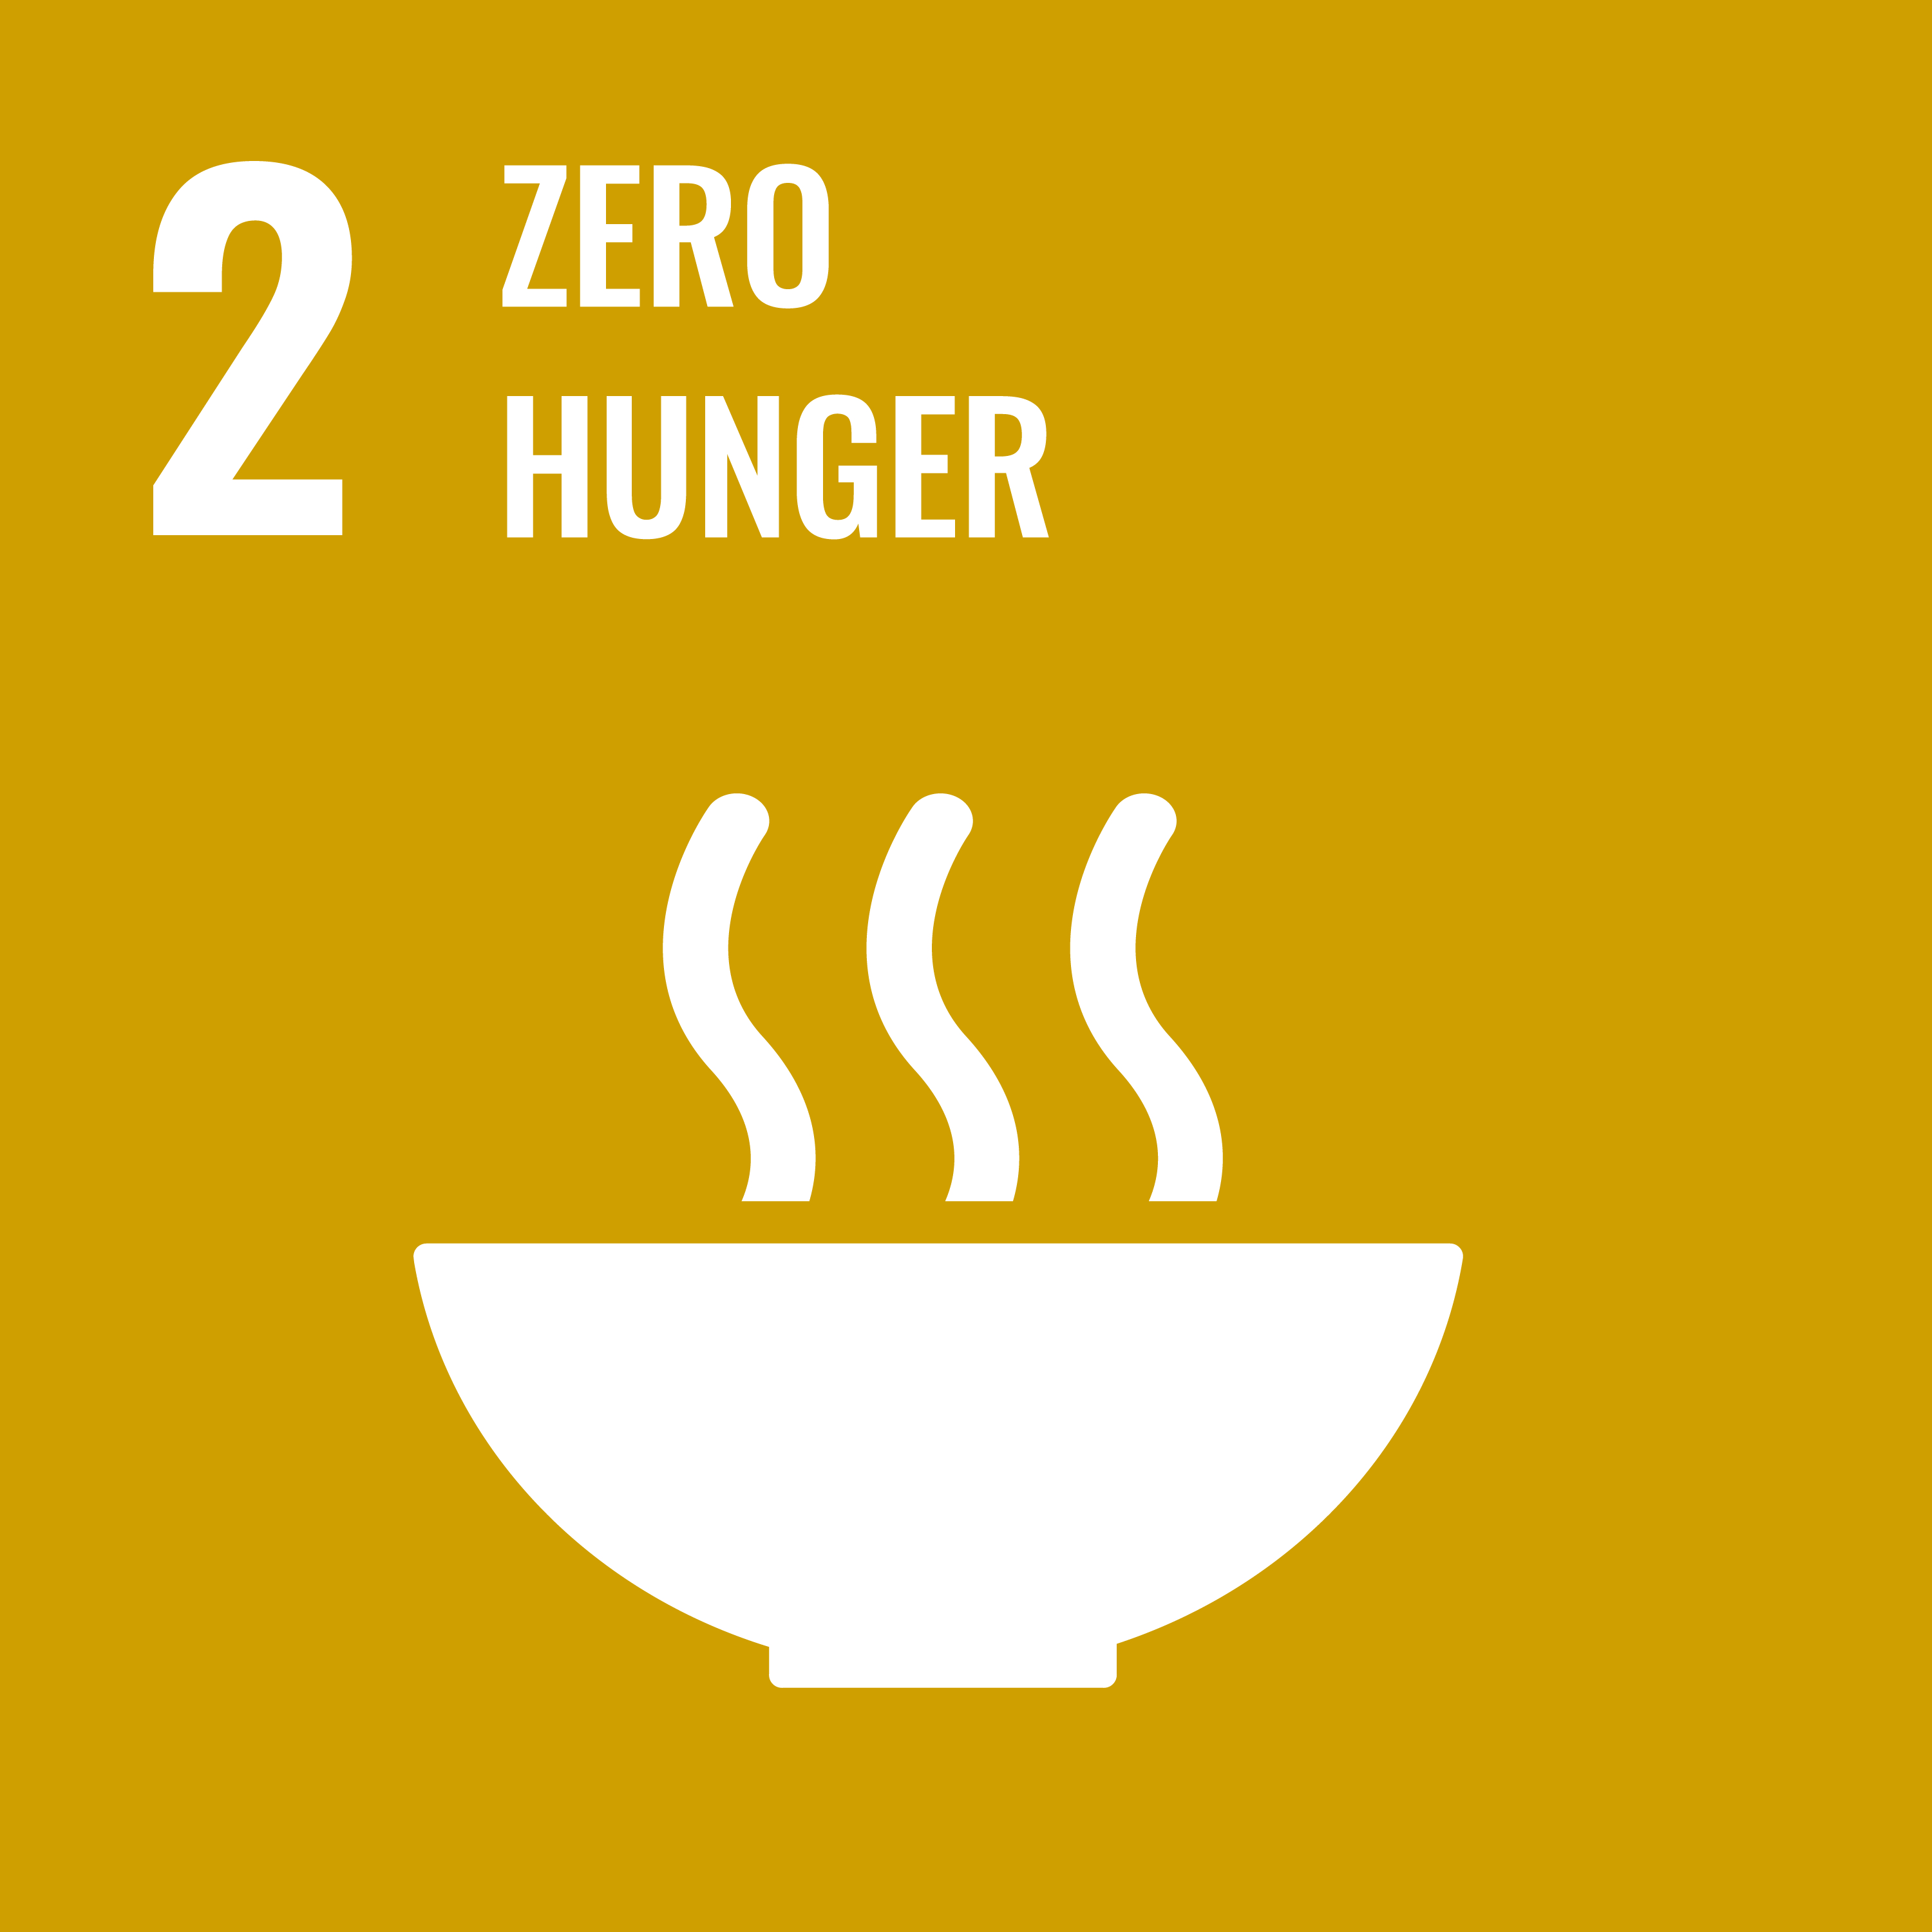
\includegraphics[width=0.25\linewidth]{Pictures/ODD/ODD02.jpg}%
	\hspace{0.5em}%
	\parbox[t]{0.7\linewidth}{\textbf{ODD 2 : Faim ``zéro''} -- Éliminer la faim, assurer la sécurité alimentaire, améliorer la nutrition et promouvoir l’agriculture durable.}
\end{minipage}

\vspace{1em}

\noindent
% Ligne 2
\begin{minipage}[t]{0.48\textwidth}
	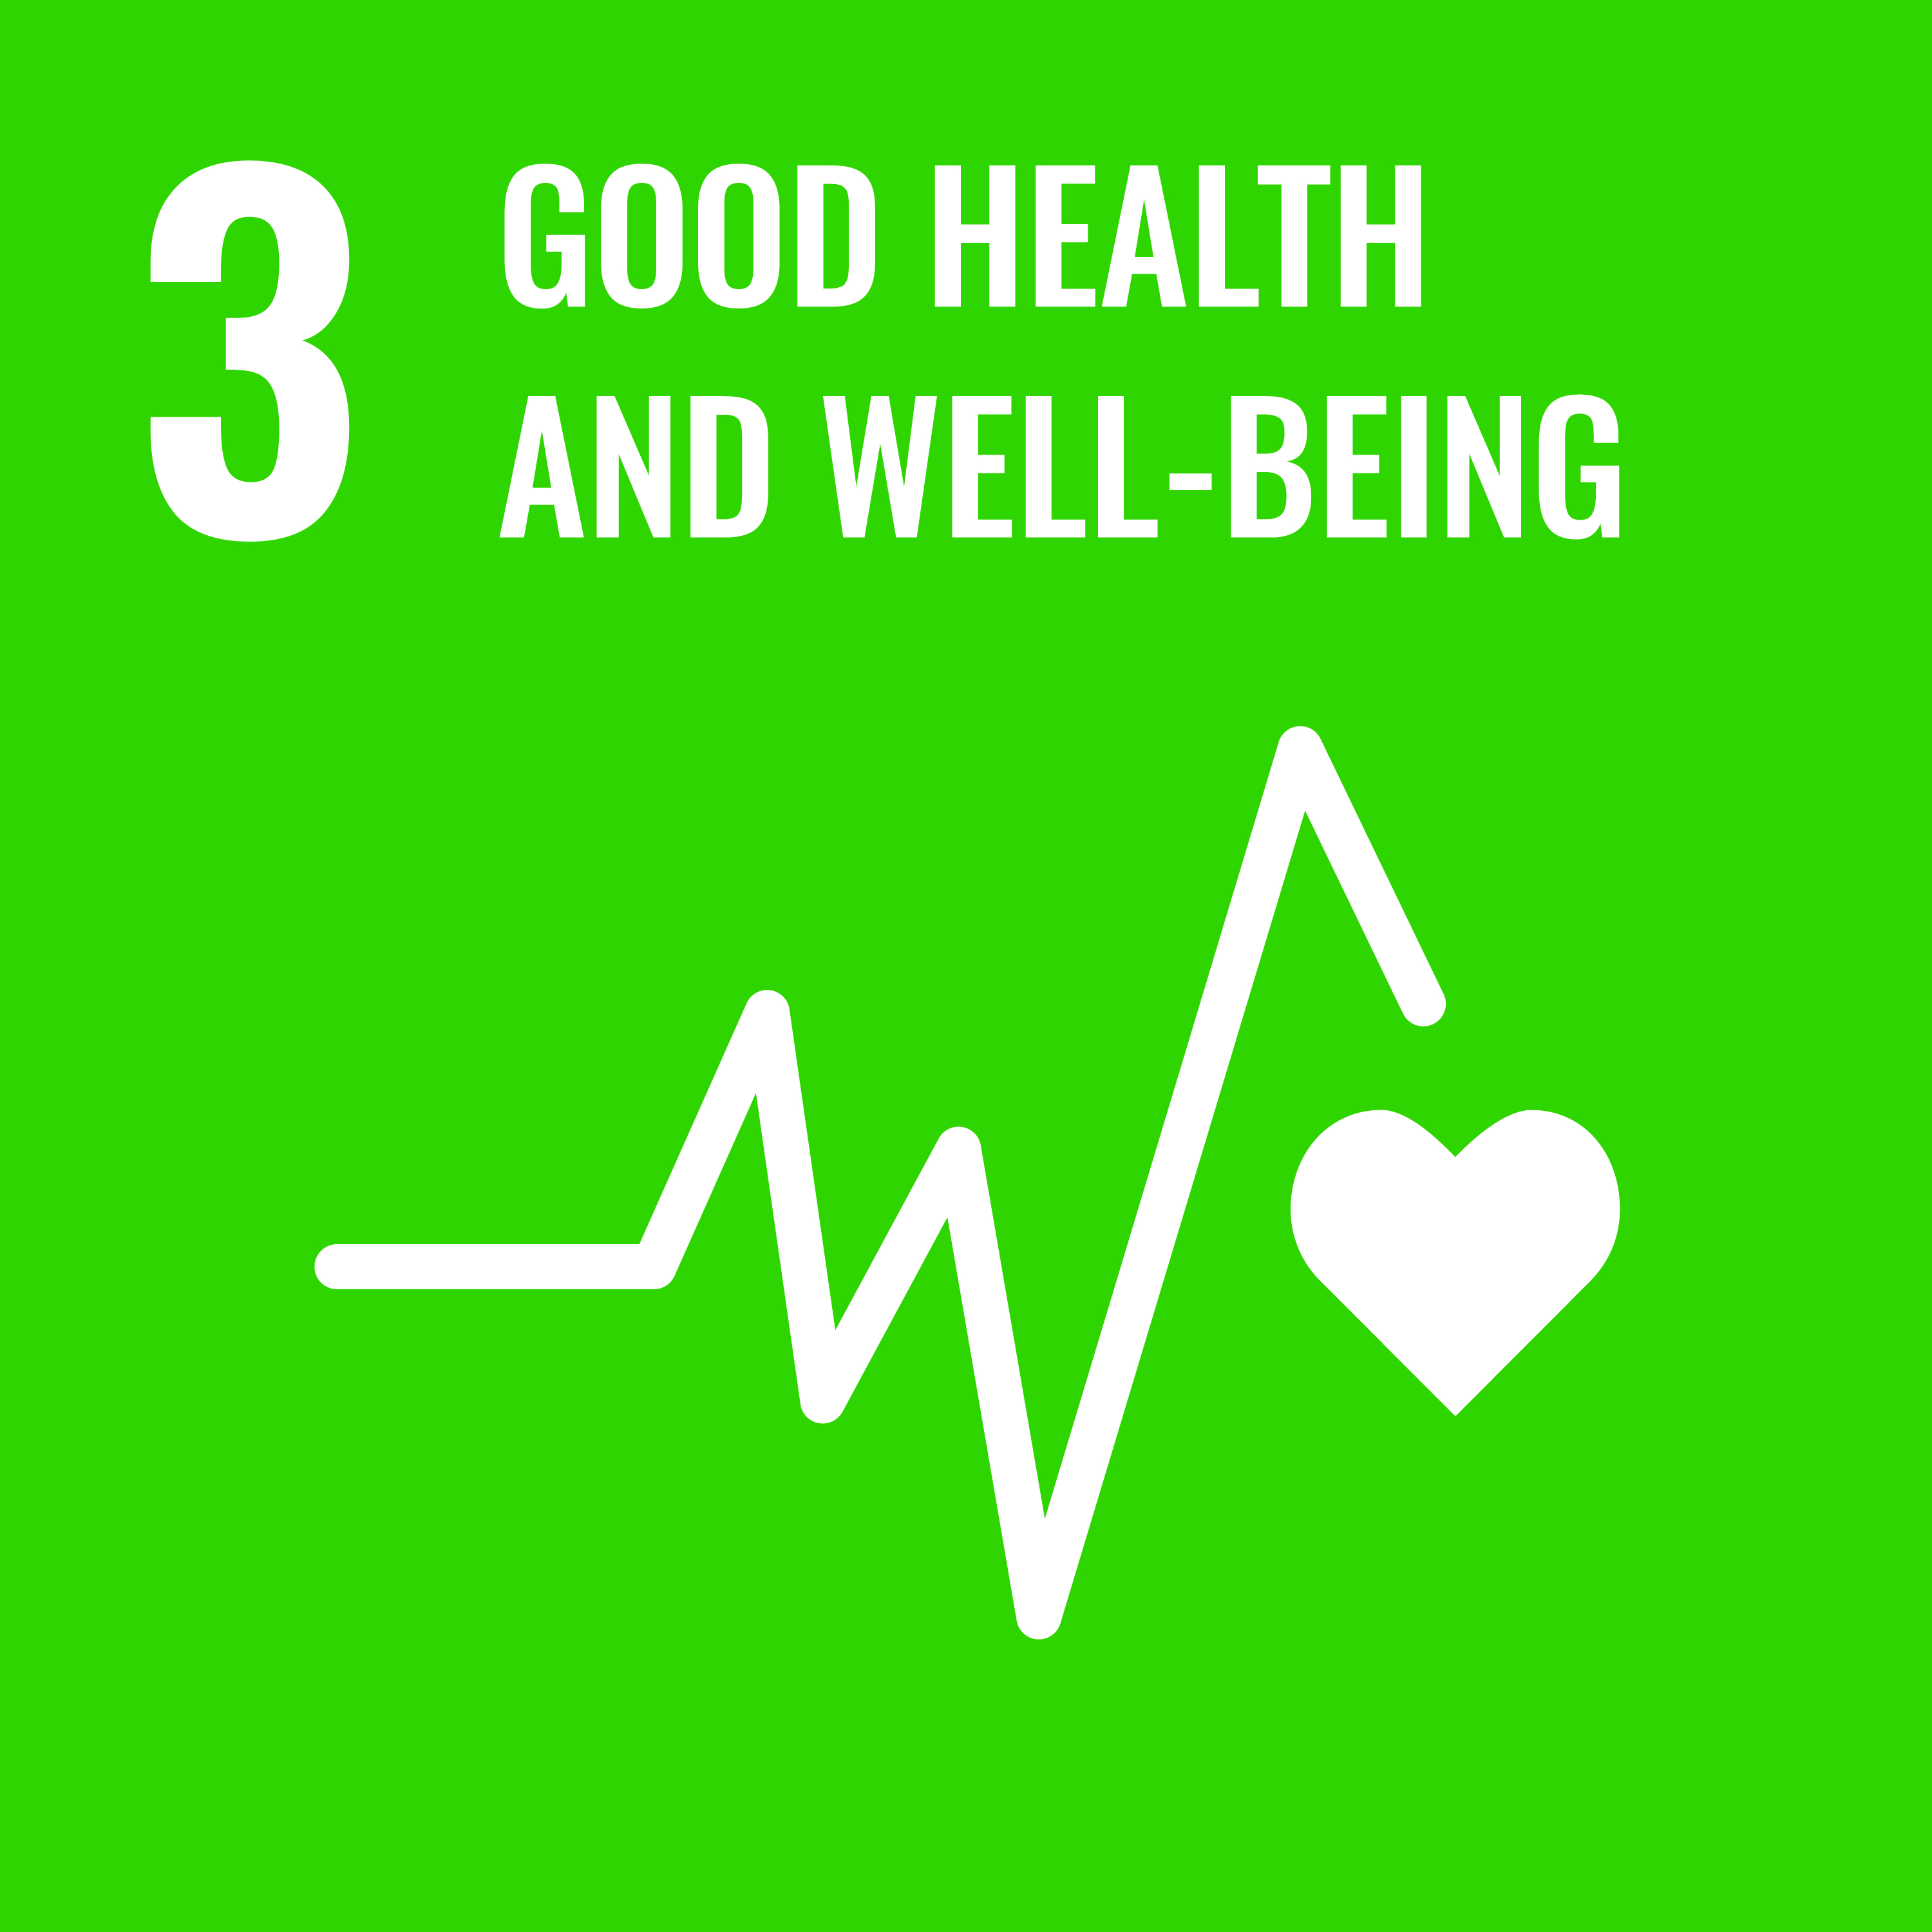
\includegraphics[width=0.25\linewidth]{Pictures/ODD/ODD03.jpg}%
	\hspace{0.5em}%
	\parbox[t]{0.7\linewidth}{\textbf{ODD 3 : Bonne santé et bien-être} -- Permettre à tous de vivre en bonne santé et promouvoir le bien-être à tout âge.}
\end{minipage}\hfill
\begin{minipage}[t]{0.48\textwidth}
	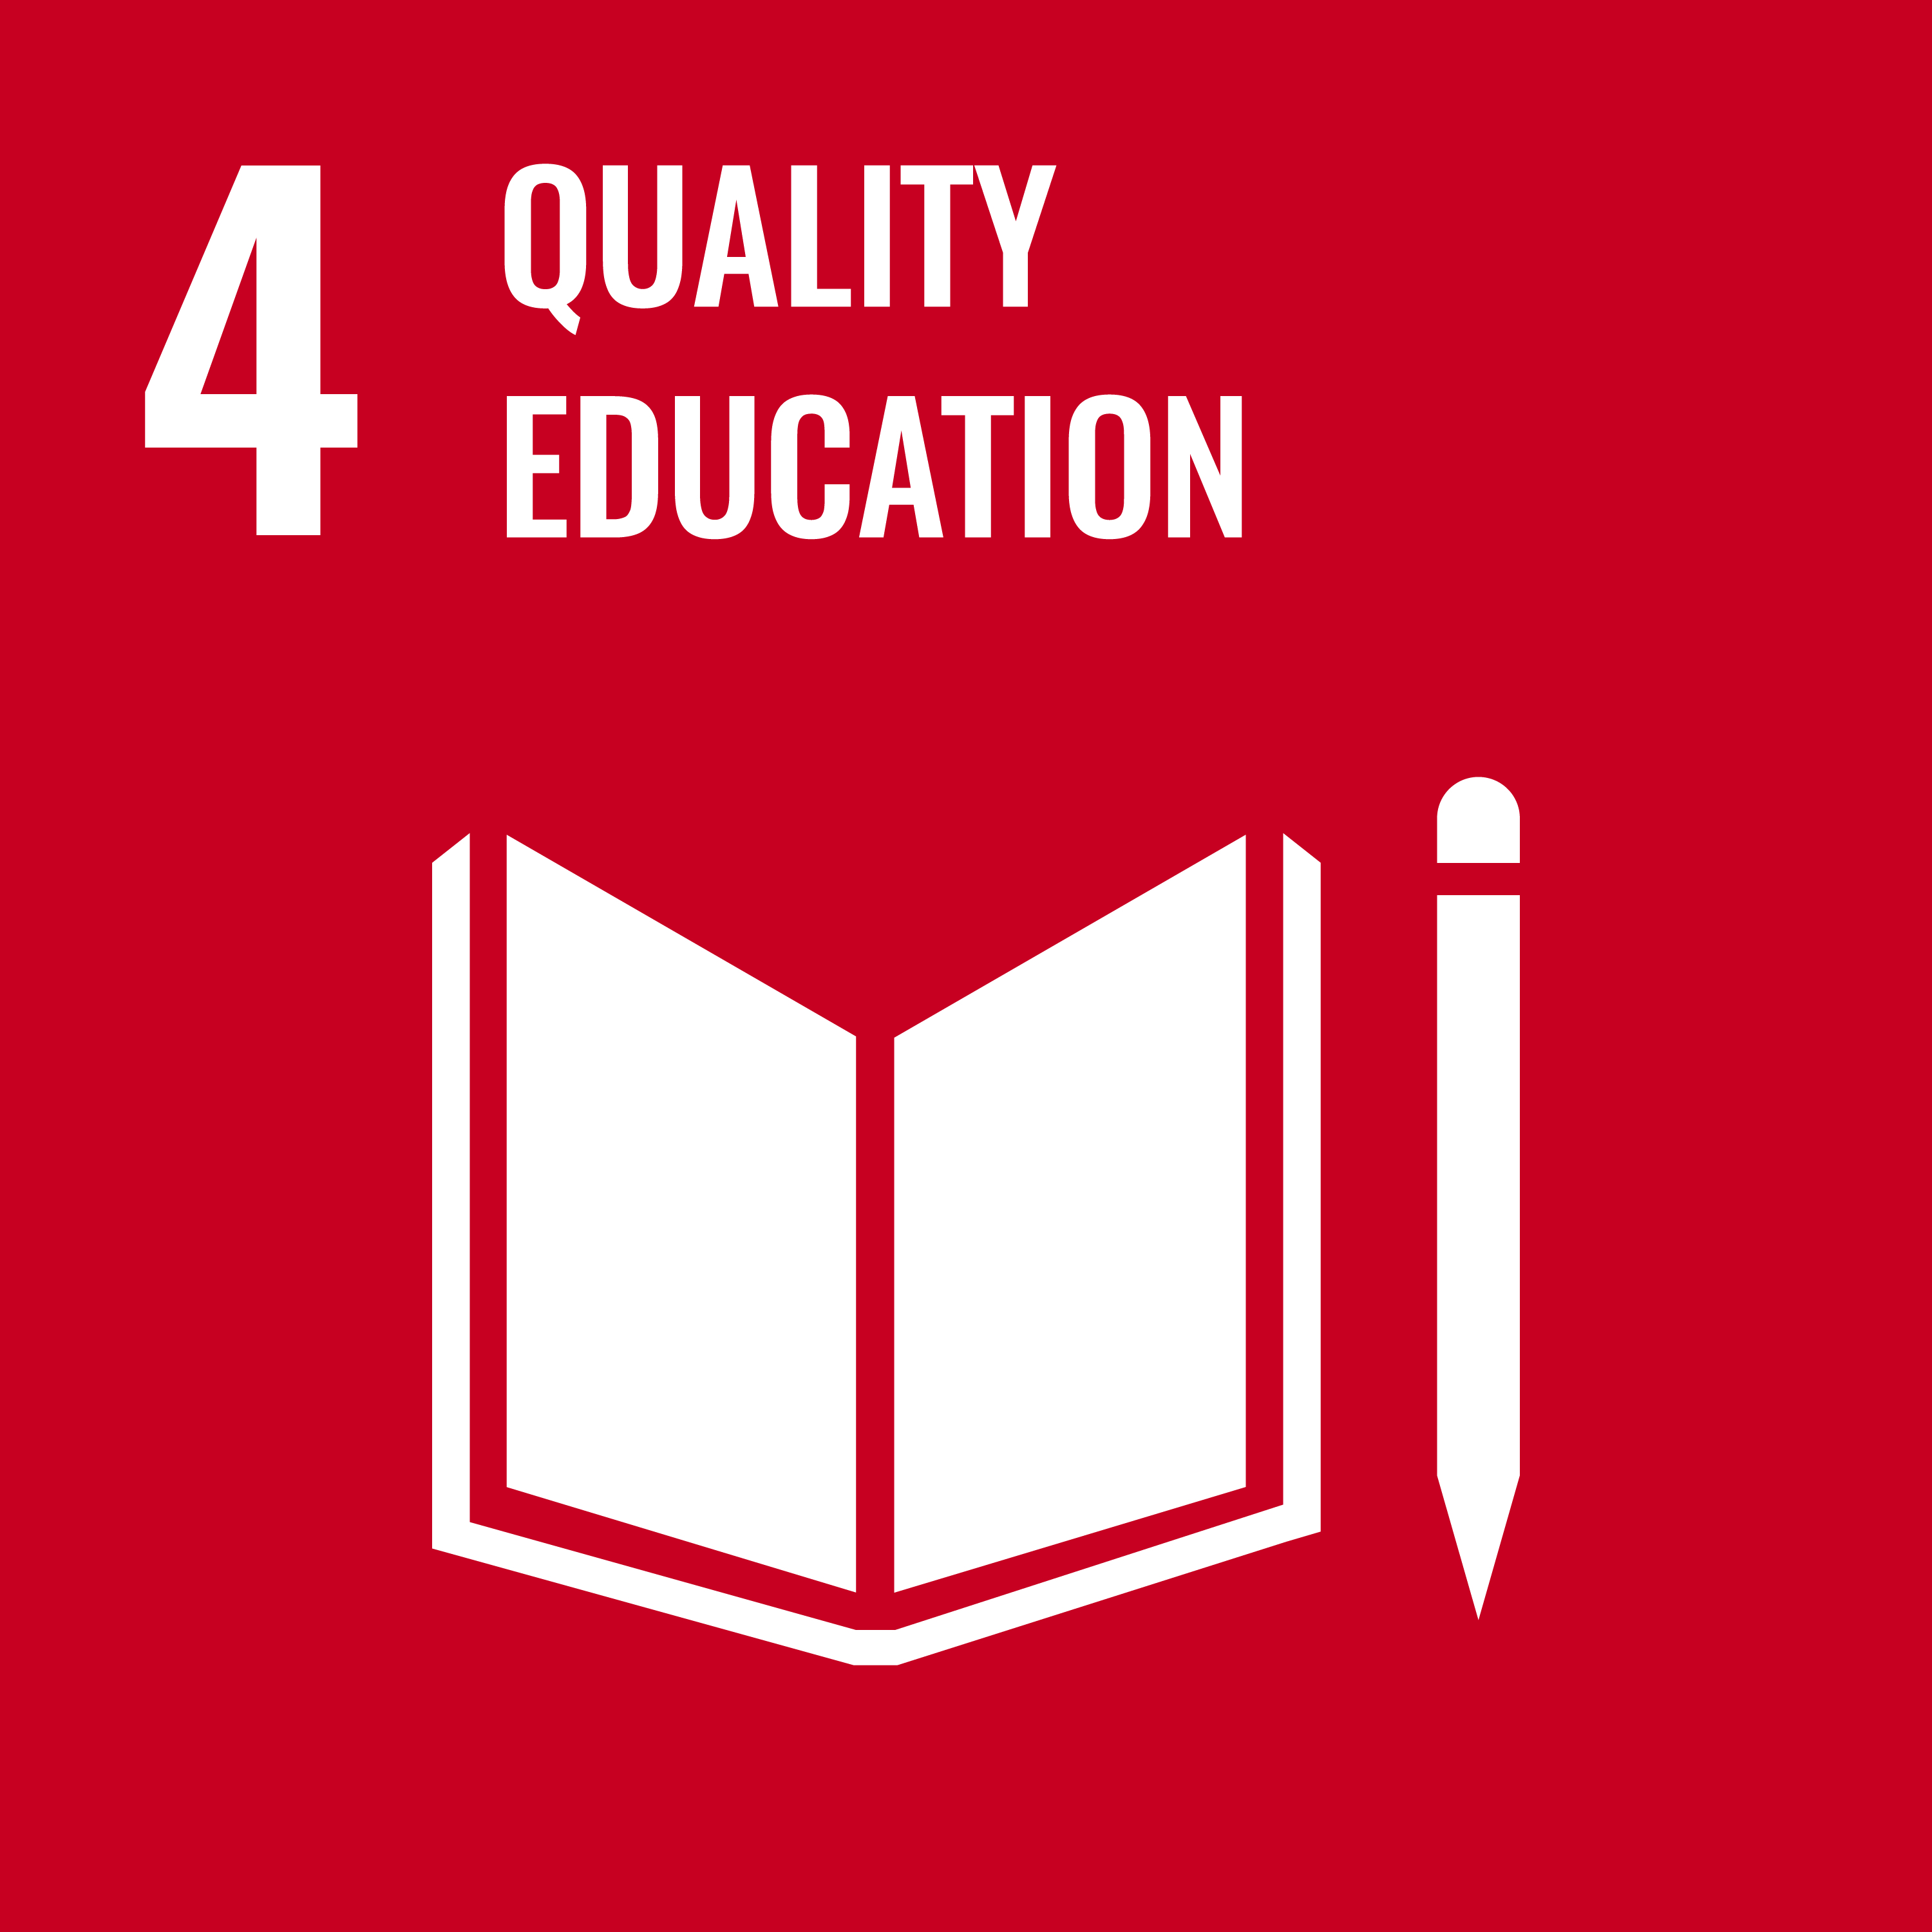
\includegraphics[width=0.25\linewidth]{Pictures/ODD/ODD04.jpg}%
	\hspace{0.5em}%
	\parbox[t]{0.7\linewidth}{\textbf{ODD 4 : Éducation de qualité} -- Assurer l’accès de tous à une éducation équitable, inclusive et de qualité et promouvoir des possibilités d’apprentissage tout au long de la vie.}
\end{minipage}

\vspace{1em}

\noindent
% Ligne 3
\begin{minipage}[t]{0.48\textwidth}
	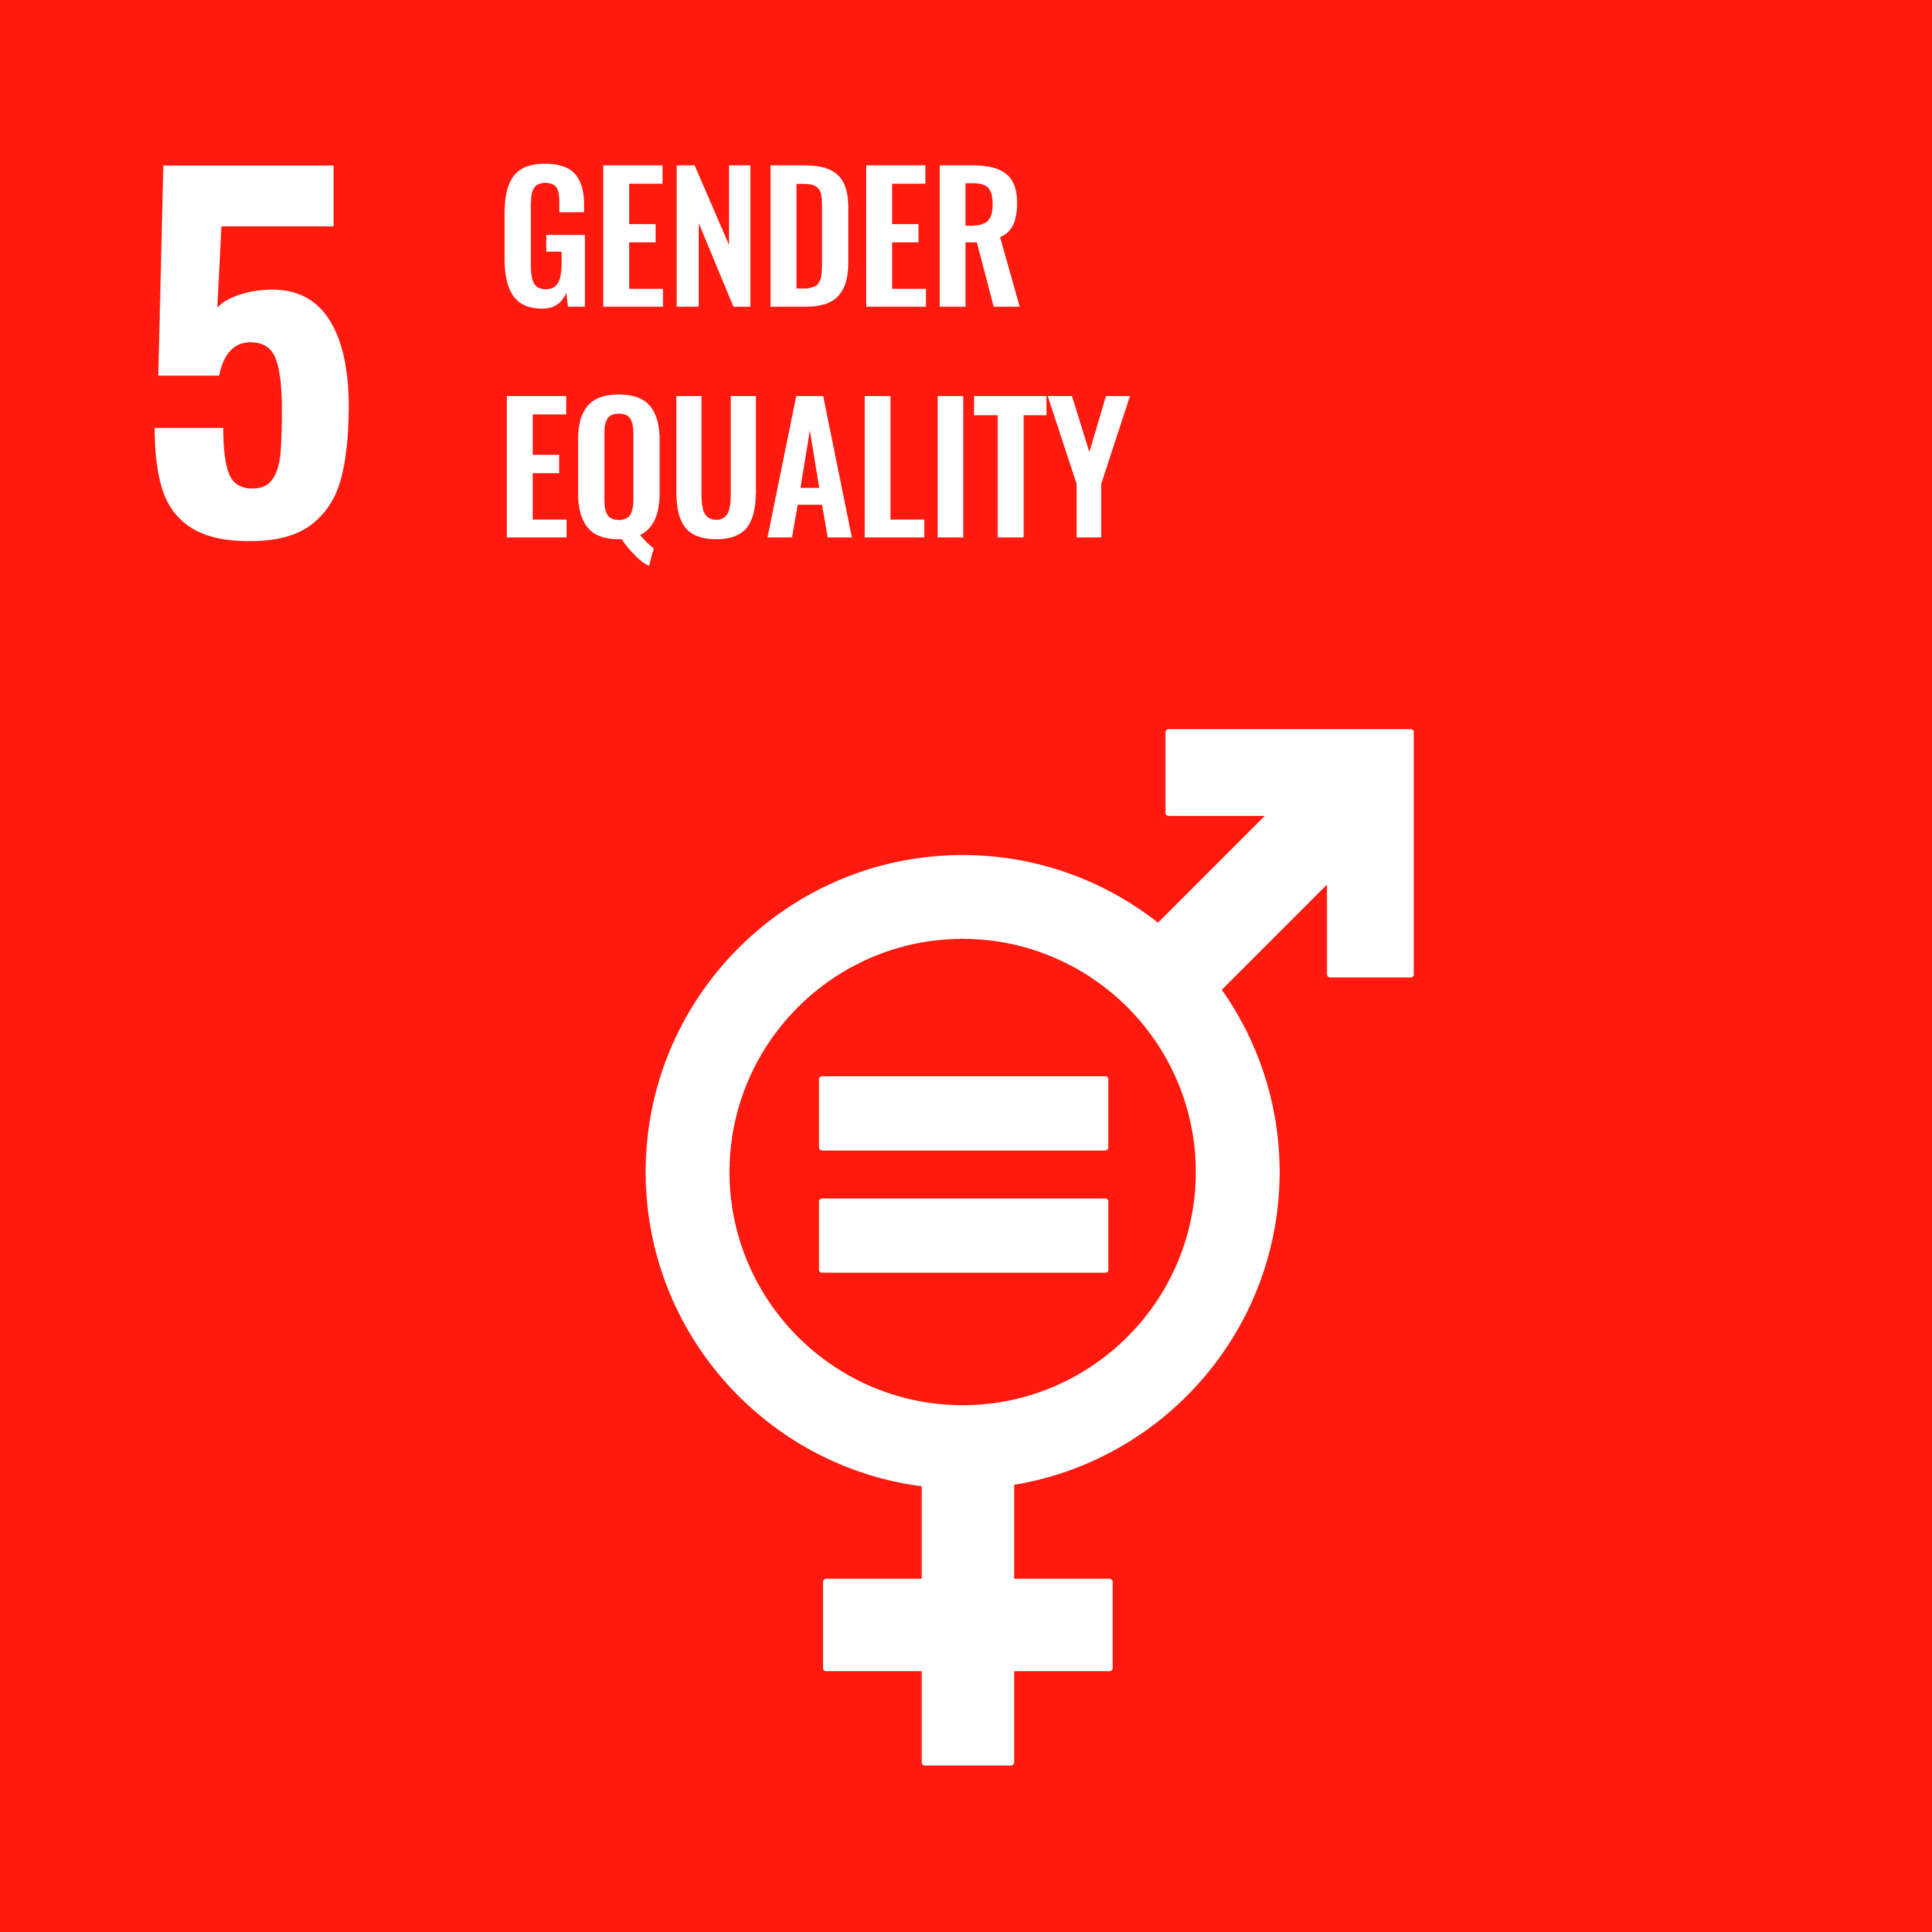
\includegraphics[width=0.25\linewidth]{Pictures/ODD/ODD05.jpg}%
	\hspace{0.5em}%
	\parbox[t]{0.7\linewidth}{\textbf{ODD 5 : Égalité entre les sexes} -- Parvenir à l’égalité des sexes et autonomiser toutes les femmes et les filles.}
\end{minipage}\hfill
\begin{minipage}[t]{0.48\textwidth}
	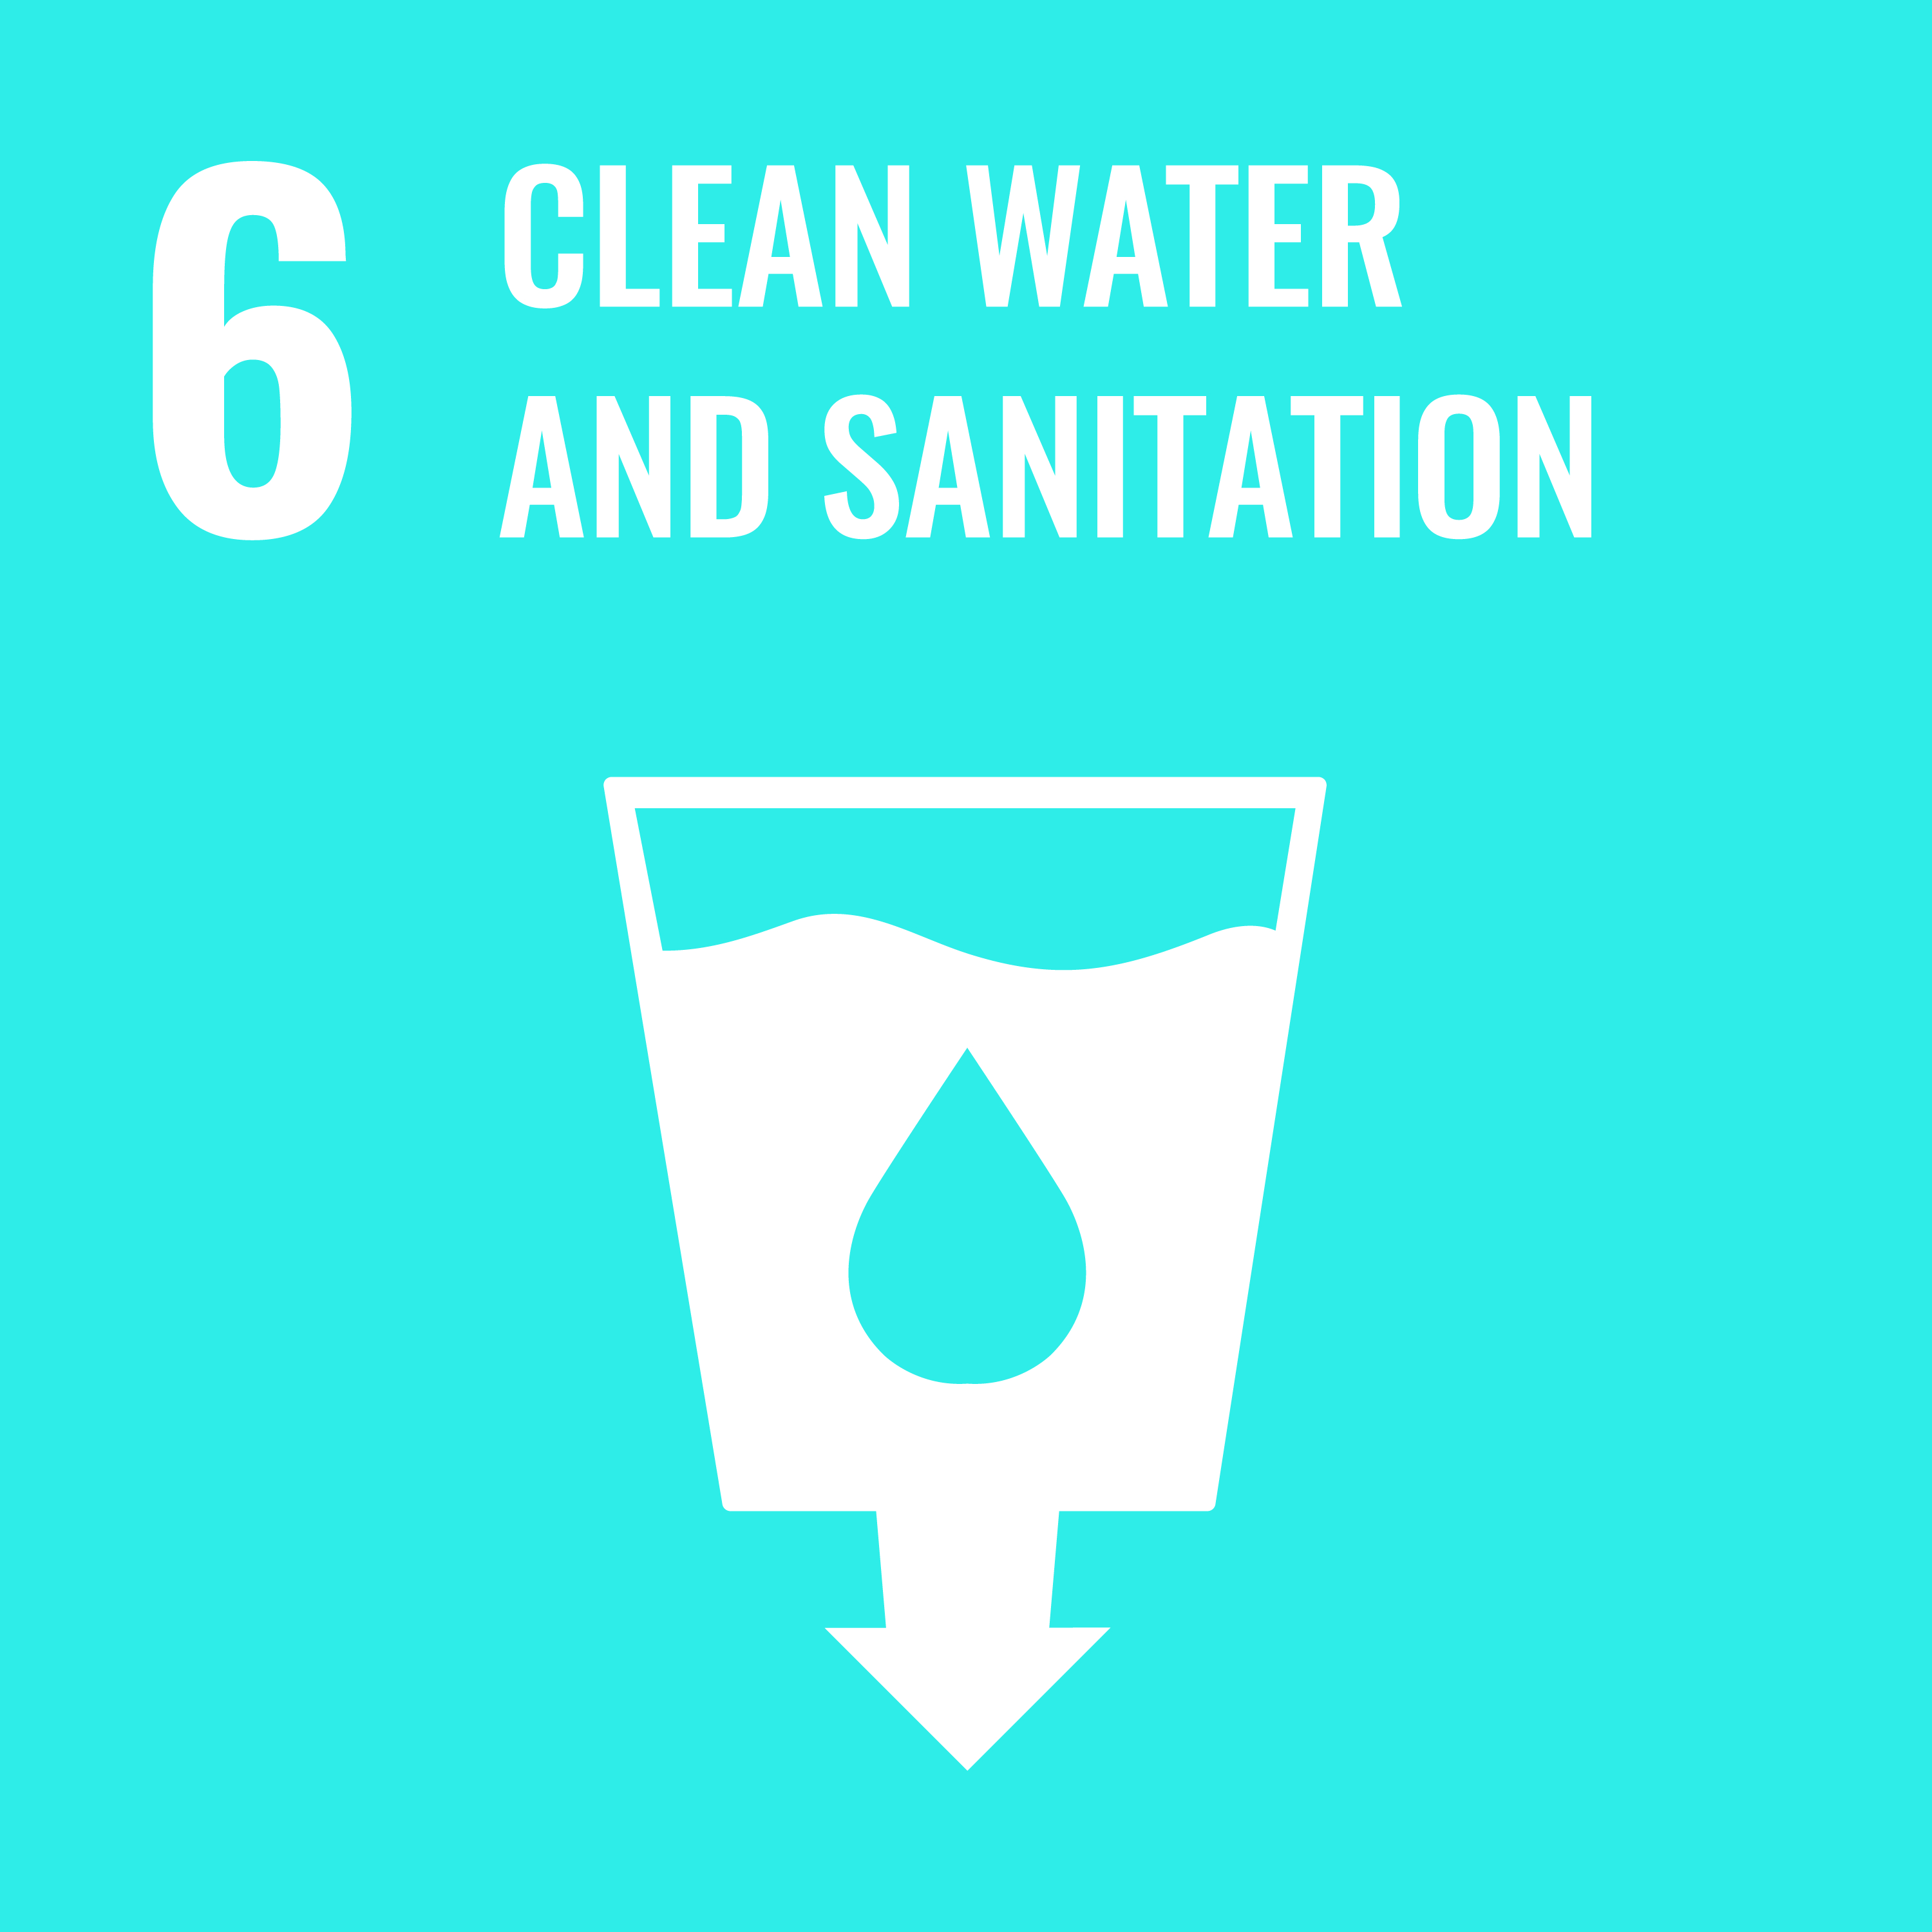
\includegraphics[width=0.25\linewidth]{Pictures/ODD/ODD06.jpg}%
	\hspace{0.5em}%
	\parbox[t]{0.7\linewidth}{\textbf{ODD 6 : Eau propre et assainissement} -- Garantir l’accès de tous à l’eau et à l’assainissement et assurer une gestion durable des ressources en eau.}
\end{minipage}

\vspace{1em}

\noindent
% Ligne 4
\begin{minipage}[t]{0.48\textwidth}
	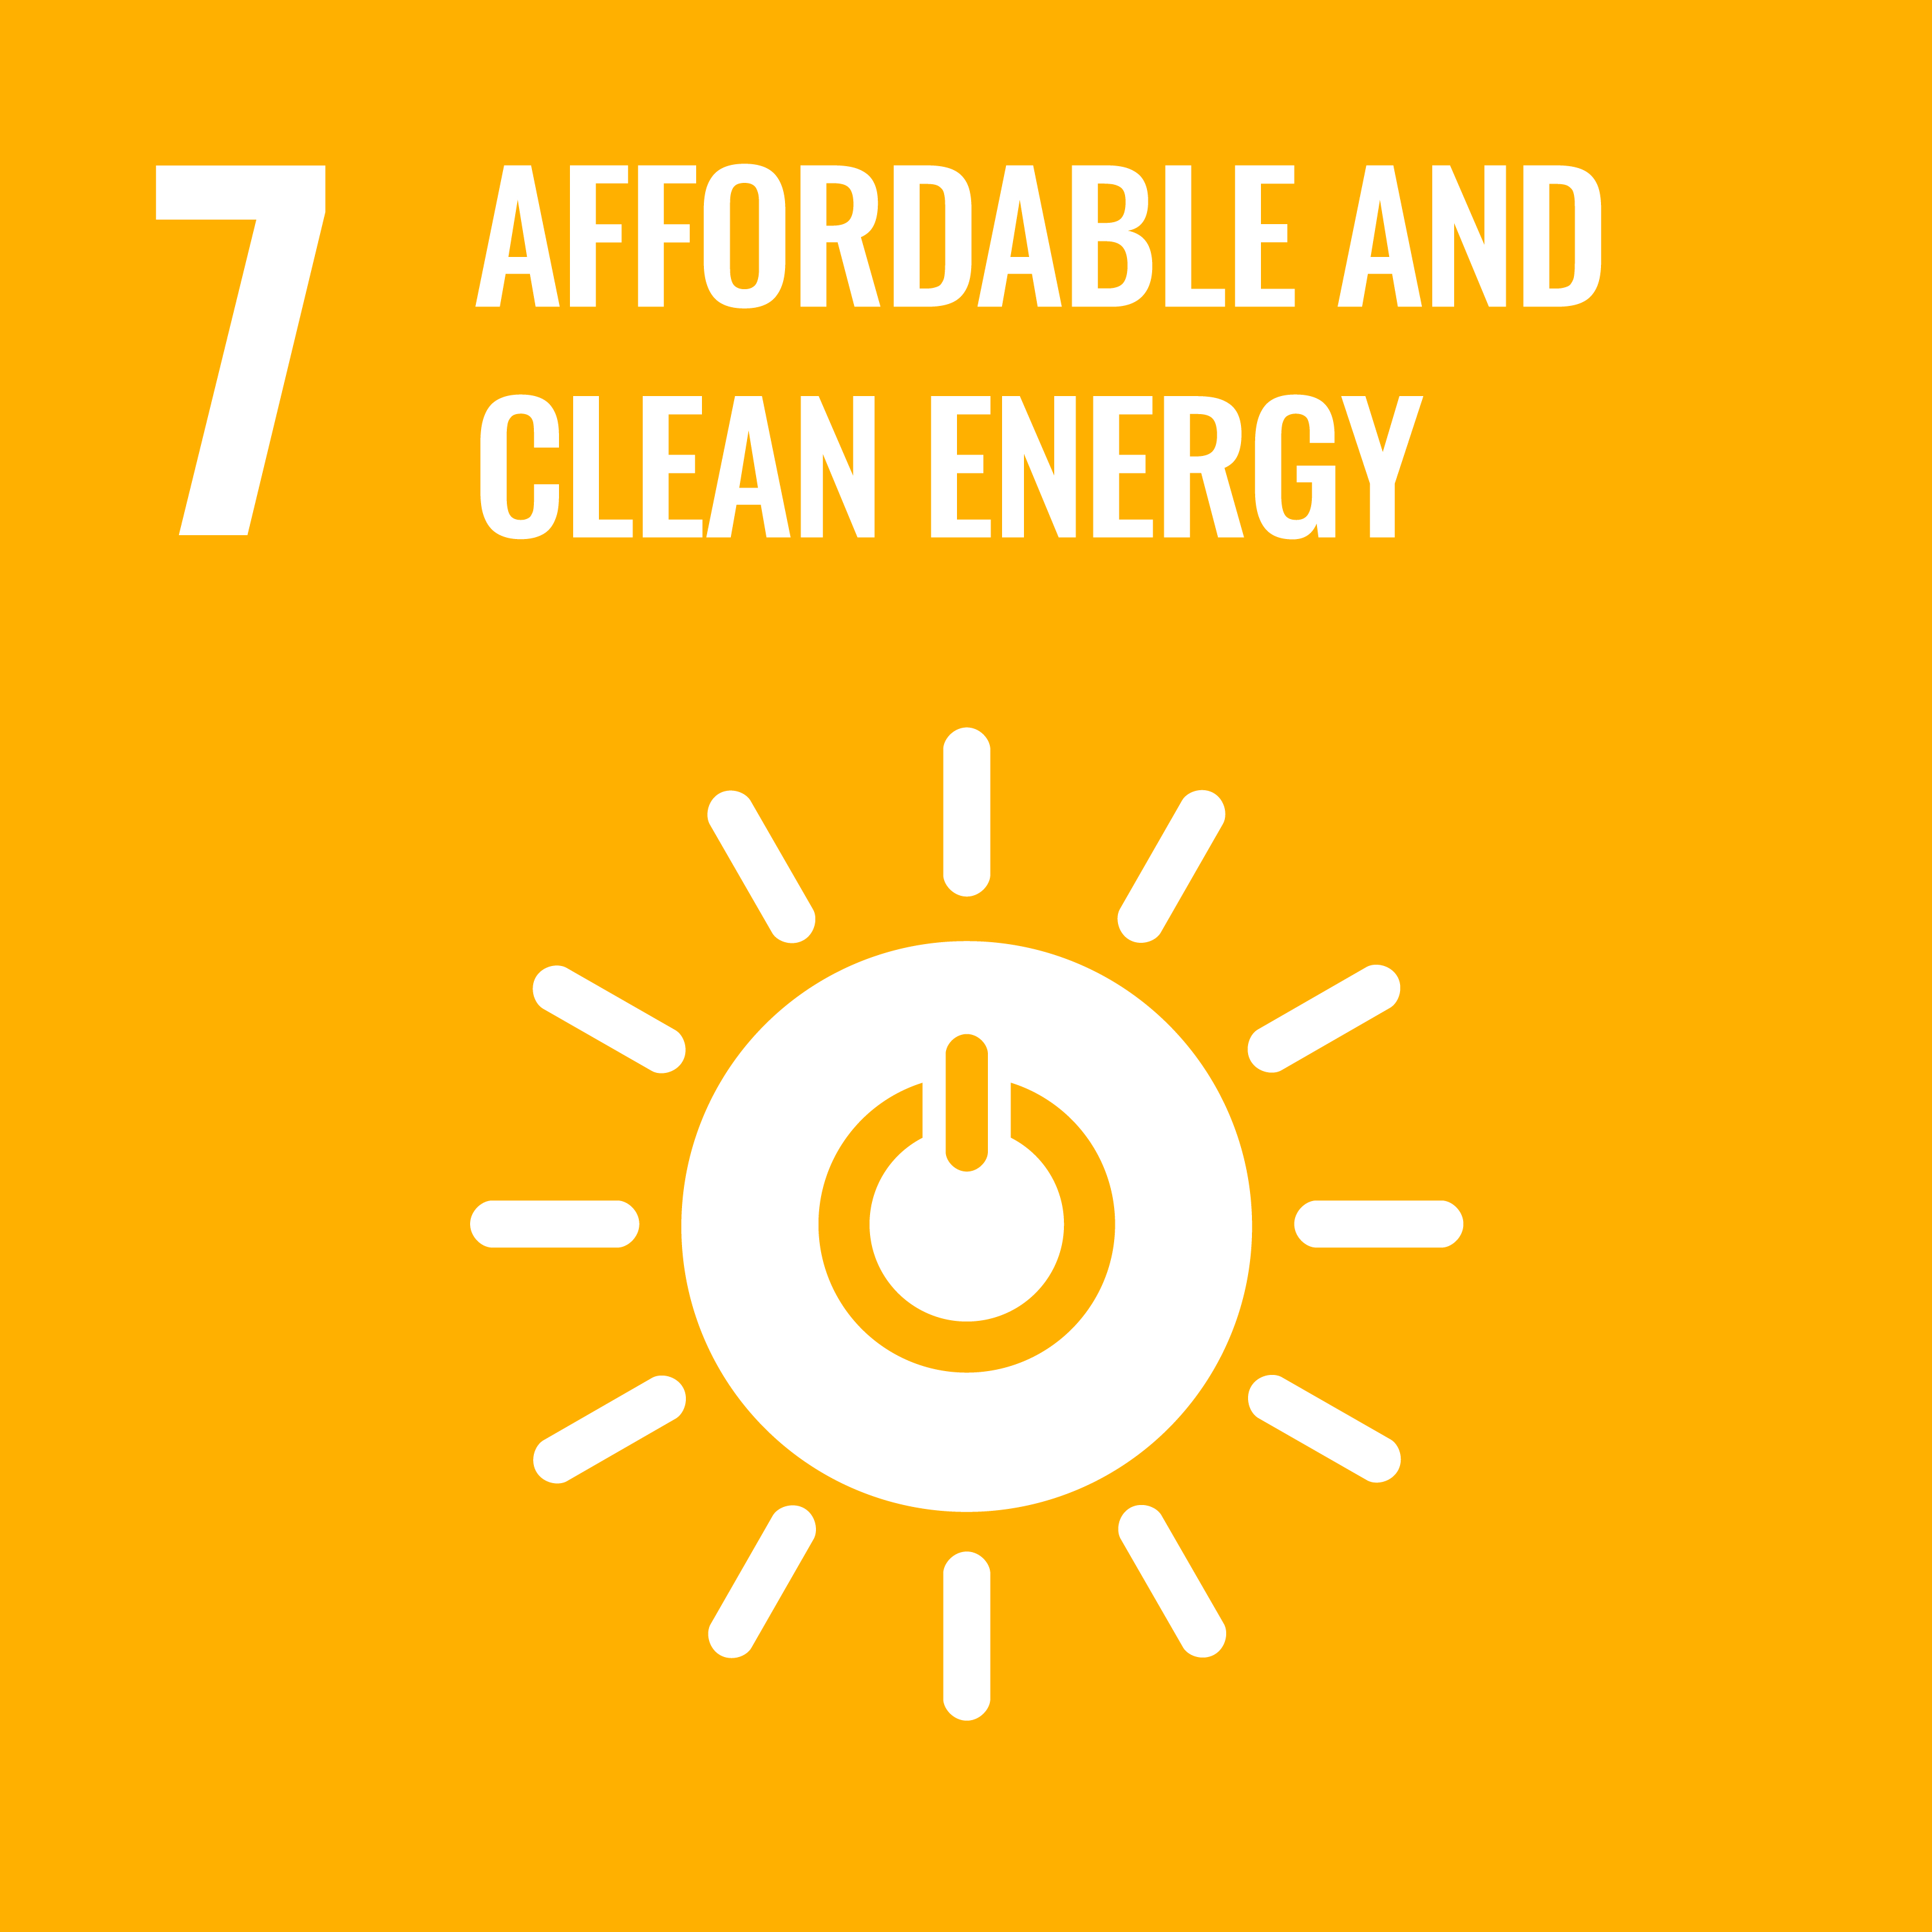
\includegraphics[width=0.25\linewidth]{Pictures/ODD/ODD07.jpg}%
	\hspace{0.5em}%
	\parbox[t]{0.7\linewidth}{\textbf{ODD 7 : Énergie propre et d’un coût abordable} -- Garantir l’accès de tous à des services énergétiques fiables, durables et modernes, à un coût abordable.}
\end{minipage}\hfill
\begin{minipage}[t]{0.48\textwidth}
	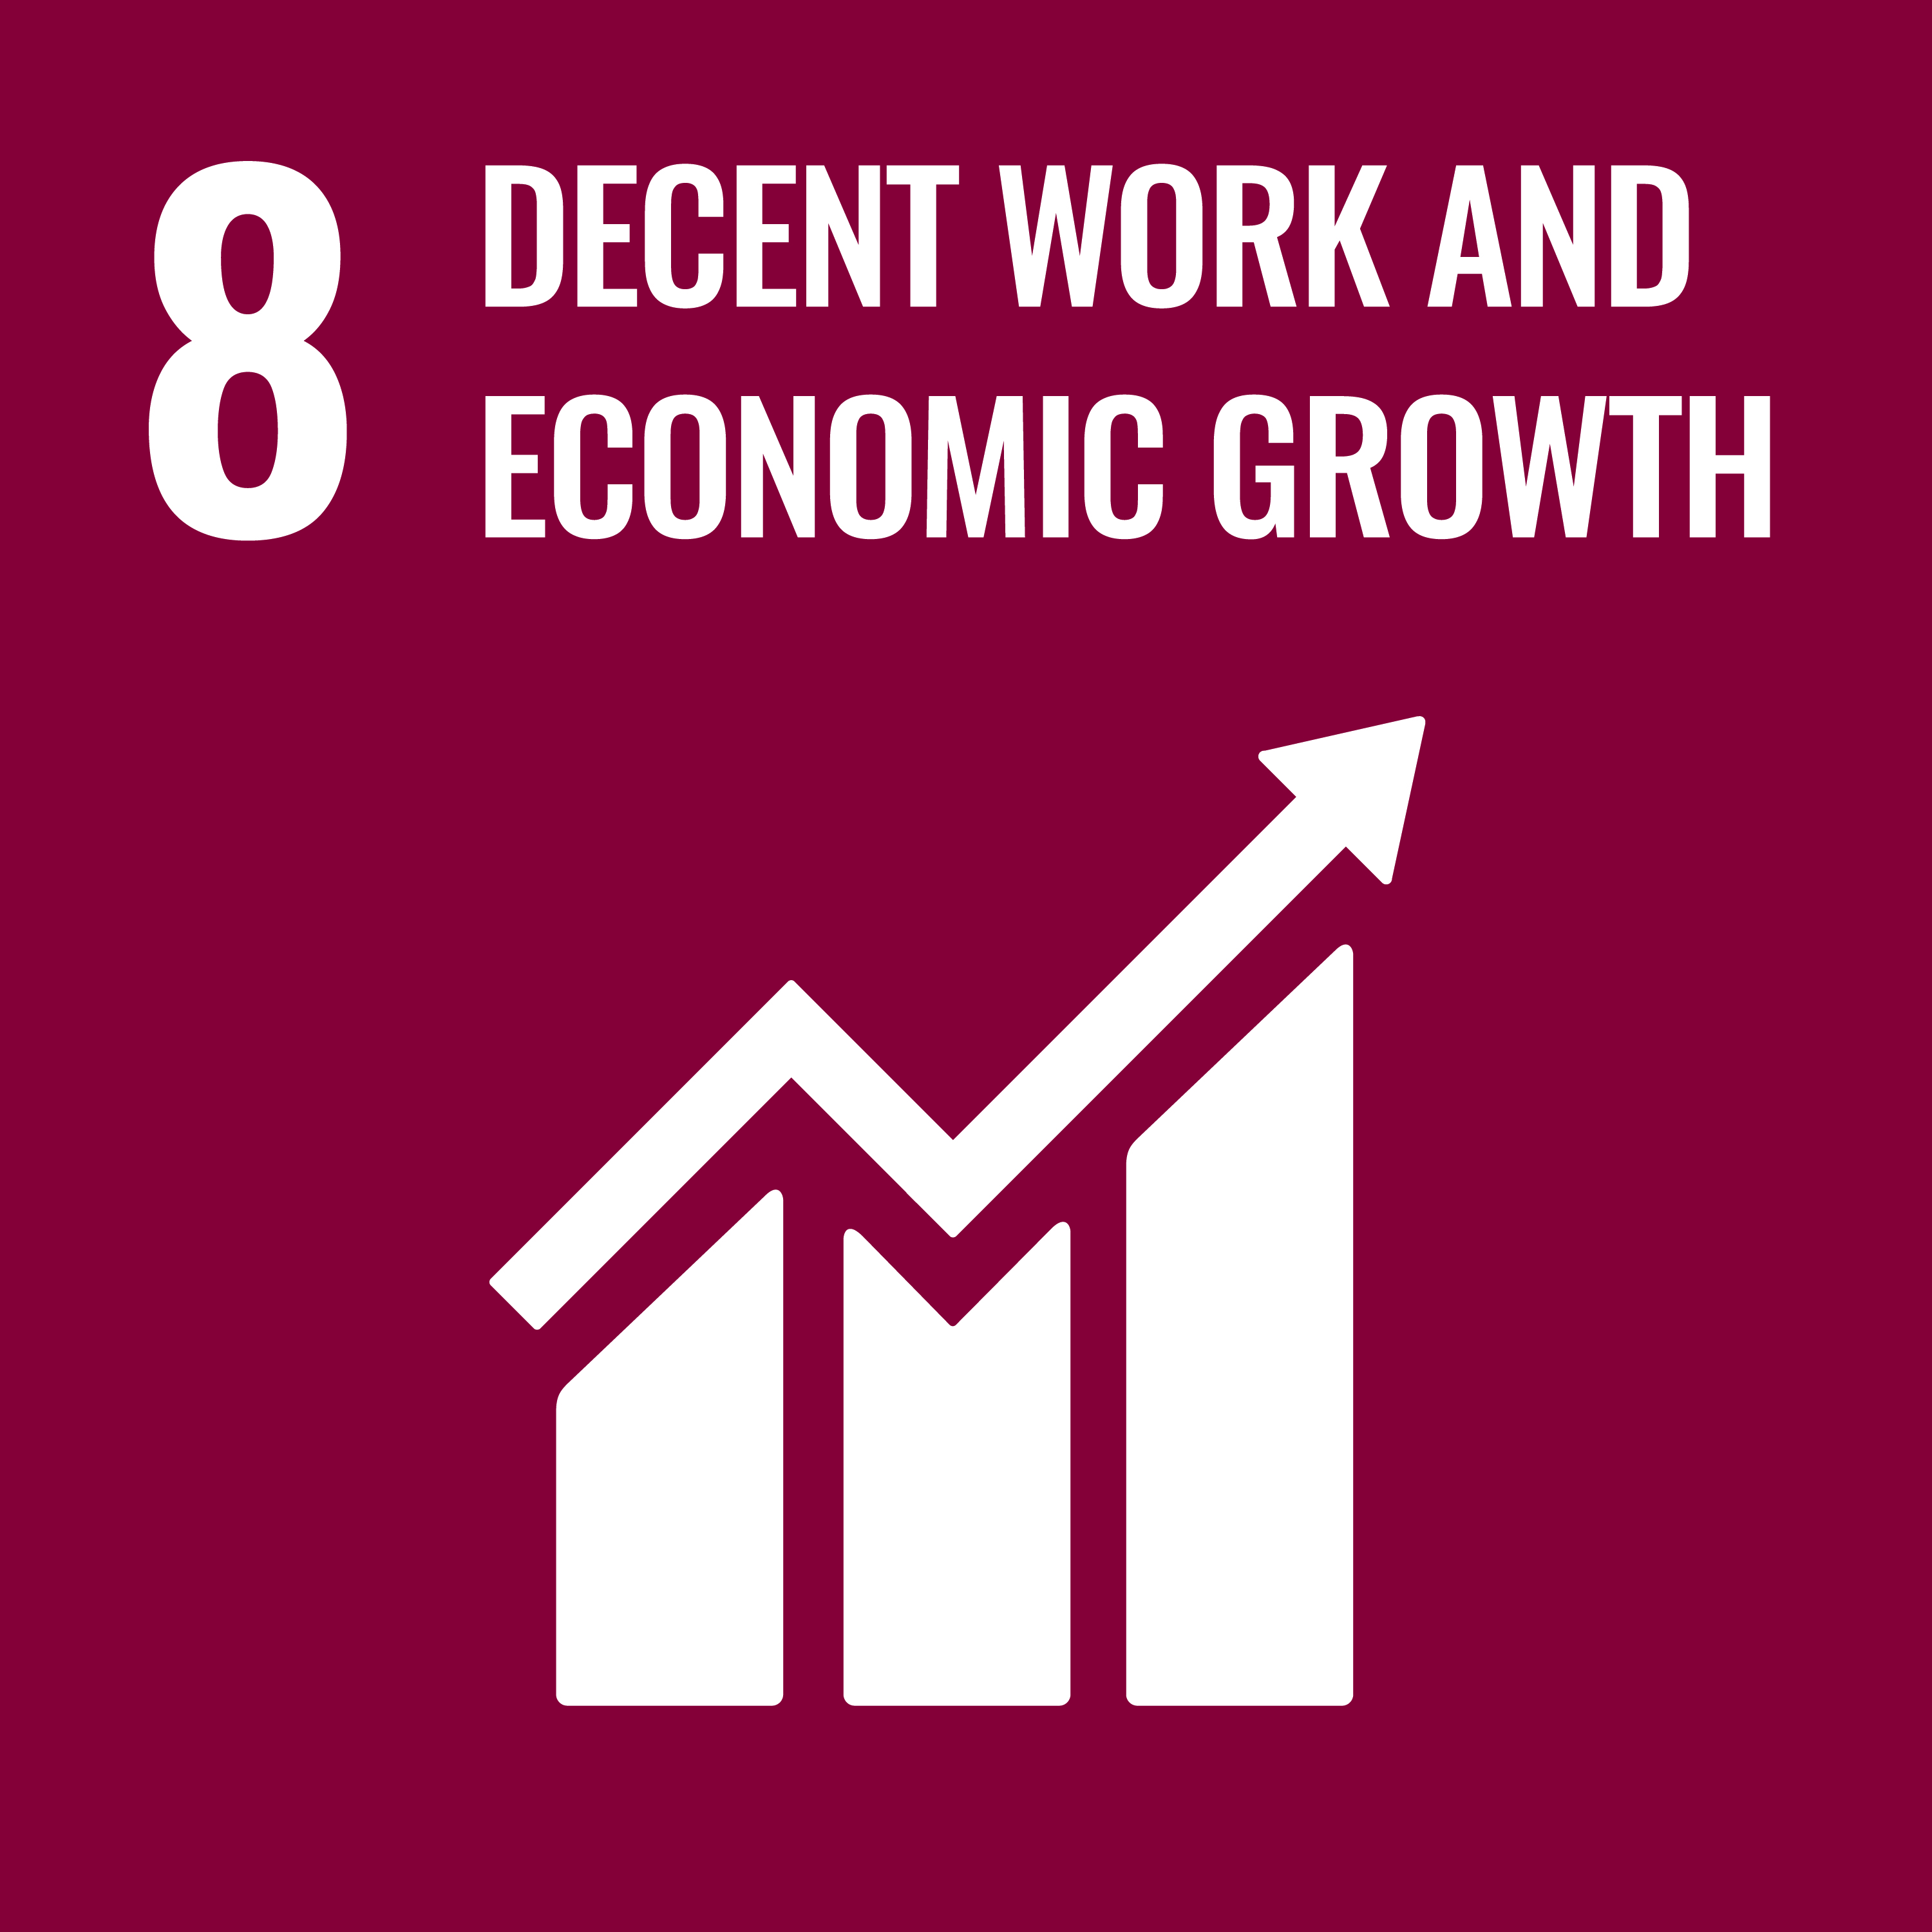
\includegraphics[width=0.25\linewidth]{Pictures/ODD/ODD08.jpg}%
	\hspace{0.5em}%
	\parbox[t]{0.7\linewidth}{\textbf{ODD 8 : Travail décent et croissance économique} -- Promouvoir une croissance économique soutenue, inclusive et durable, le plein emploi productif et un travail décent pour tous.}
\end{minipage}

\vspace{1em}

\noindent
% Ligne 5
\begin{minipage}[t]{0.48\textwidth}
	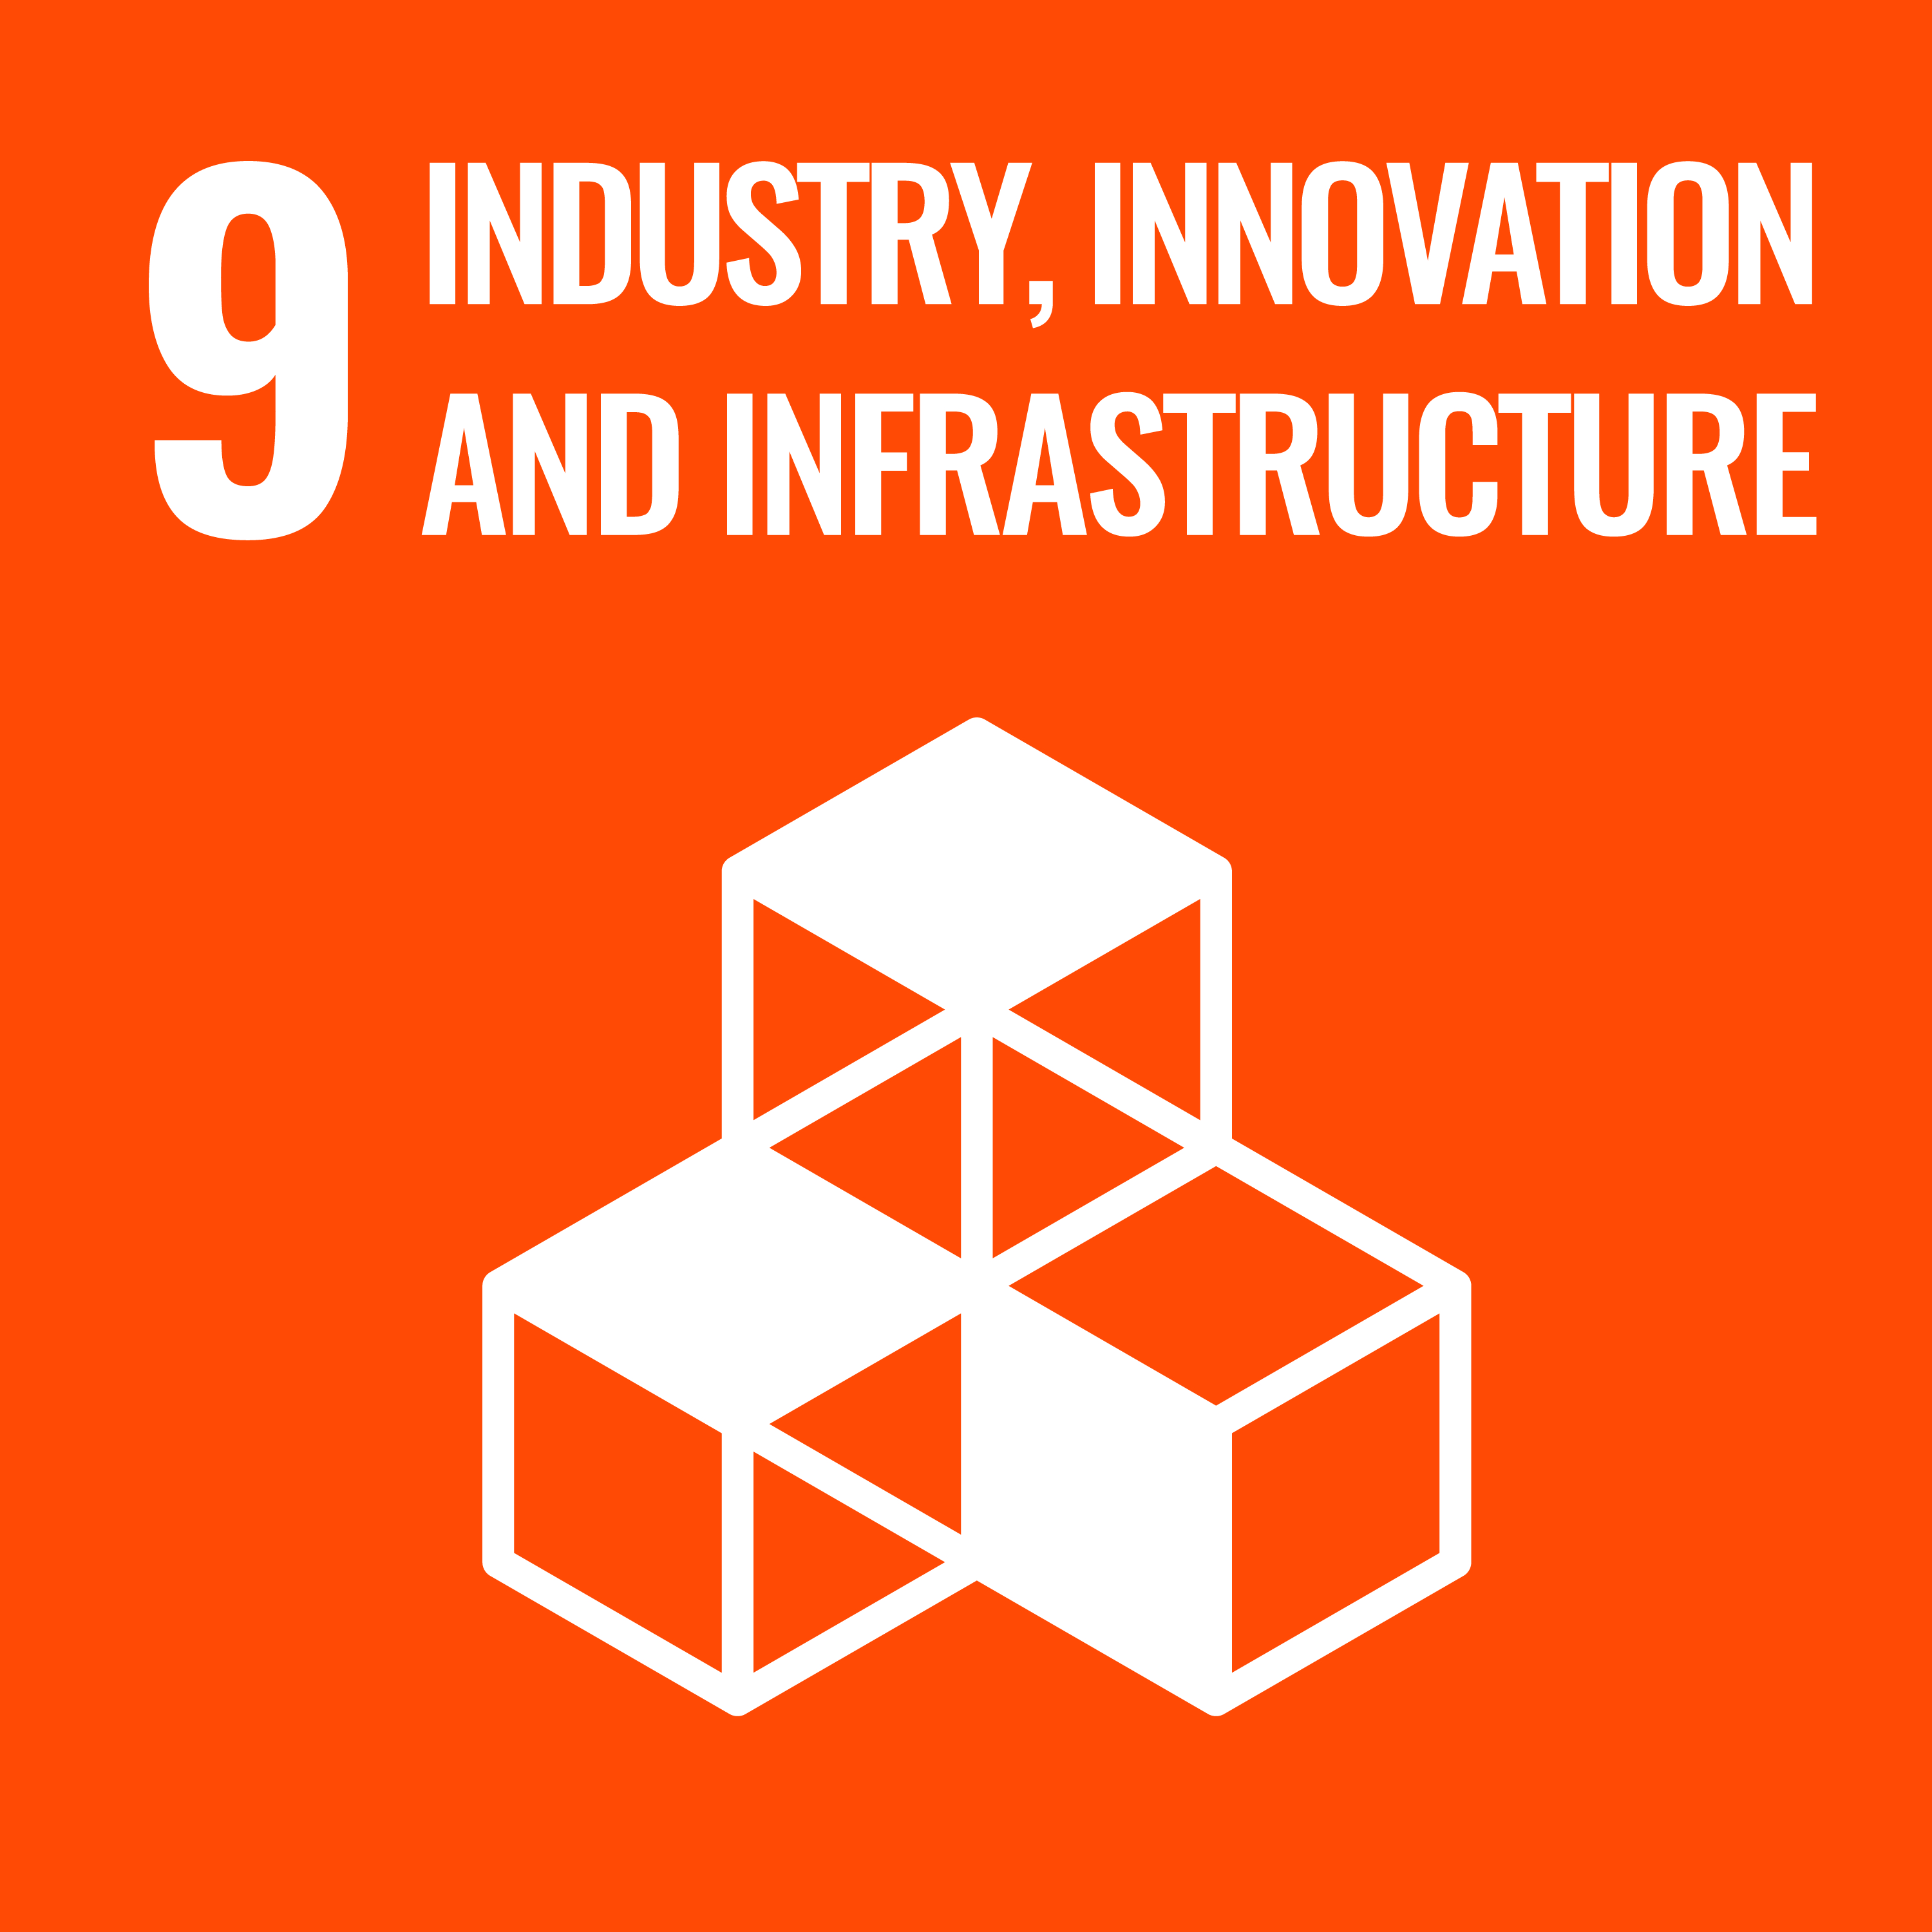
\includegraphics[width=0.25\linewidth]{Pictures/ODD/ODD09.jpg}%
	\hspace{0.5em}%
	\parbox[t]{0.7\linewidth}{\textbf{ODD 9 : Industrie, innovation et infrastructures} -- Bâtir une infrastructure résiliente, promouvoir une industrialisation durable et encourager l’innovation.}
\end{minipage}\hfill
\begin{minipage}[t]{0.48\textwidth}
	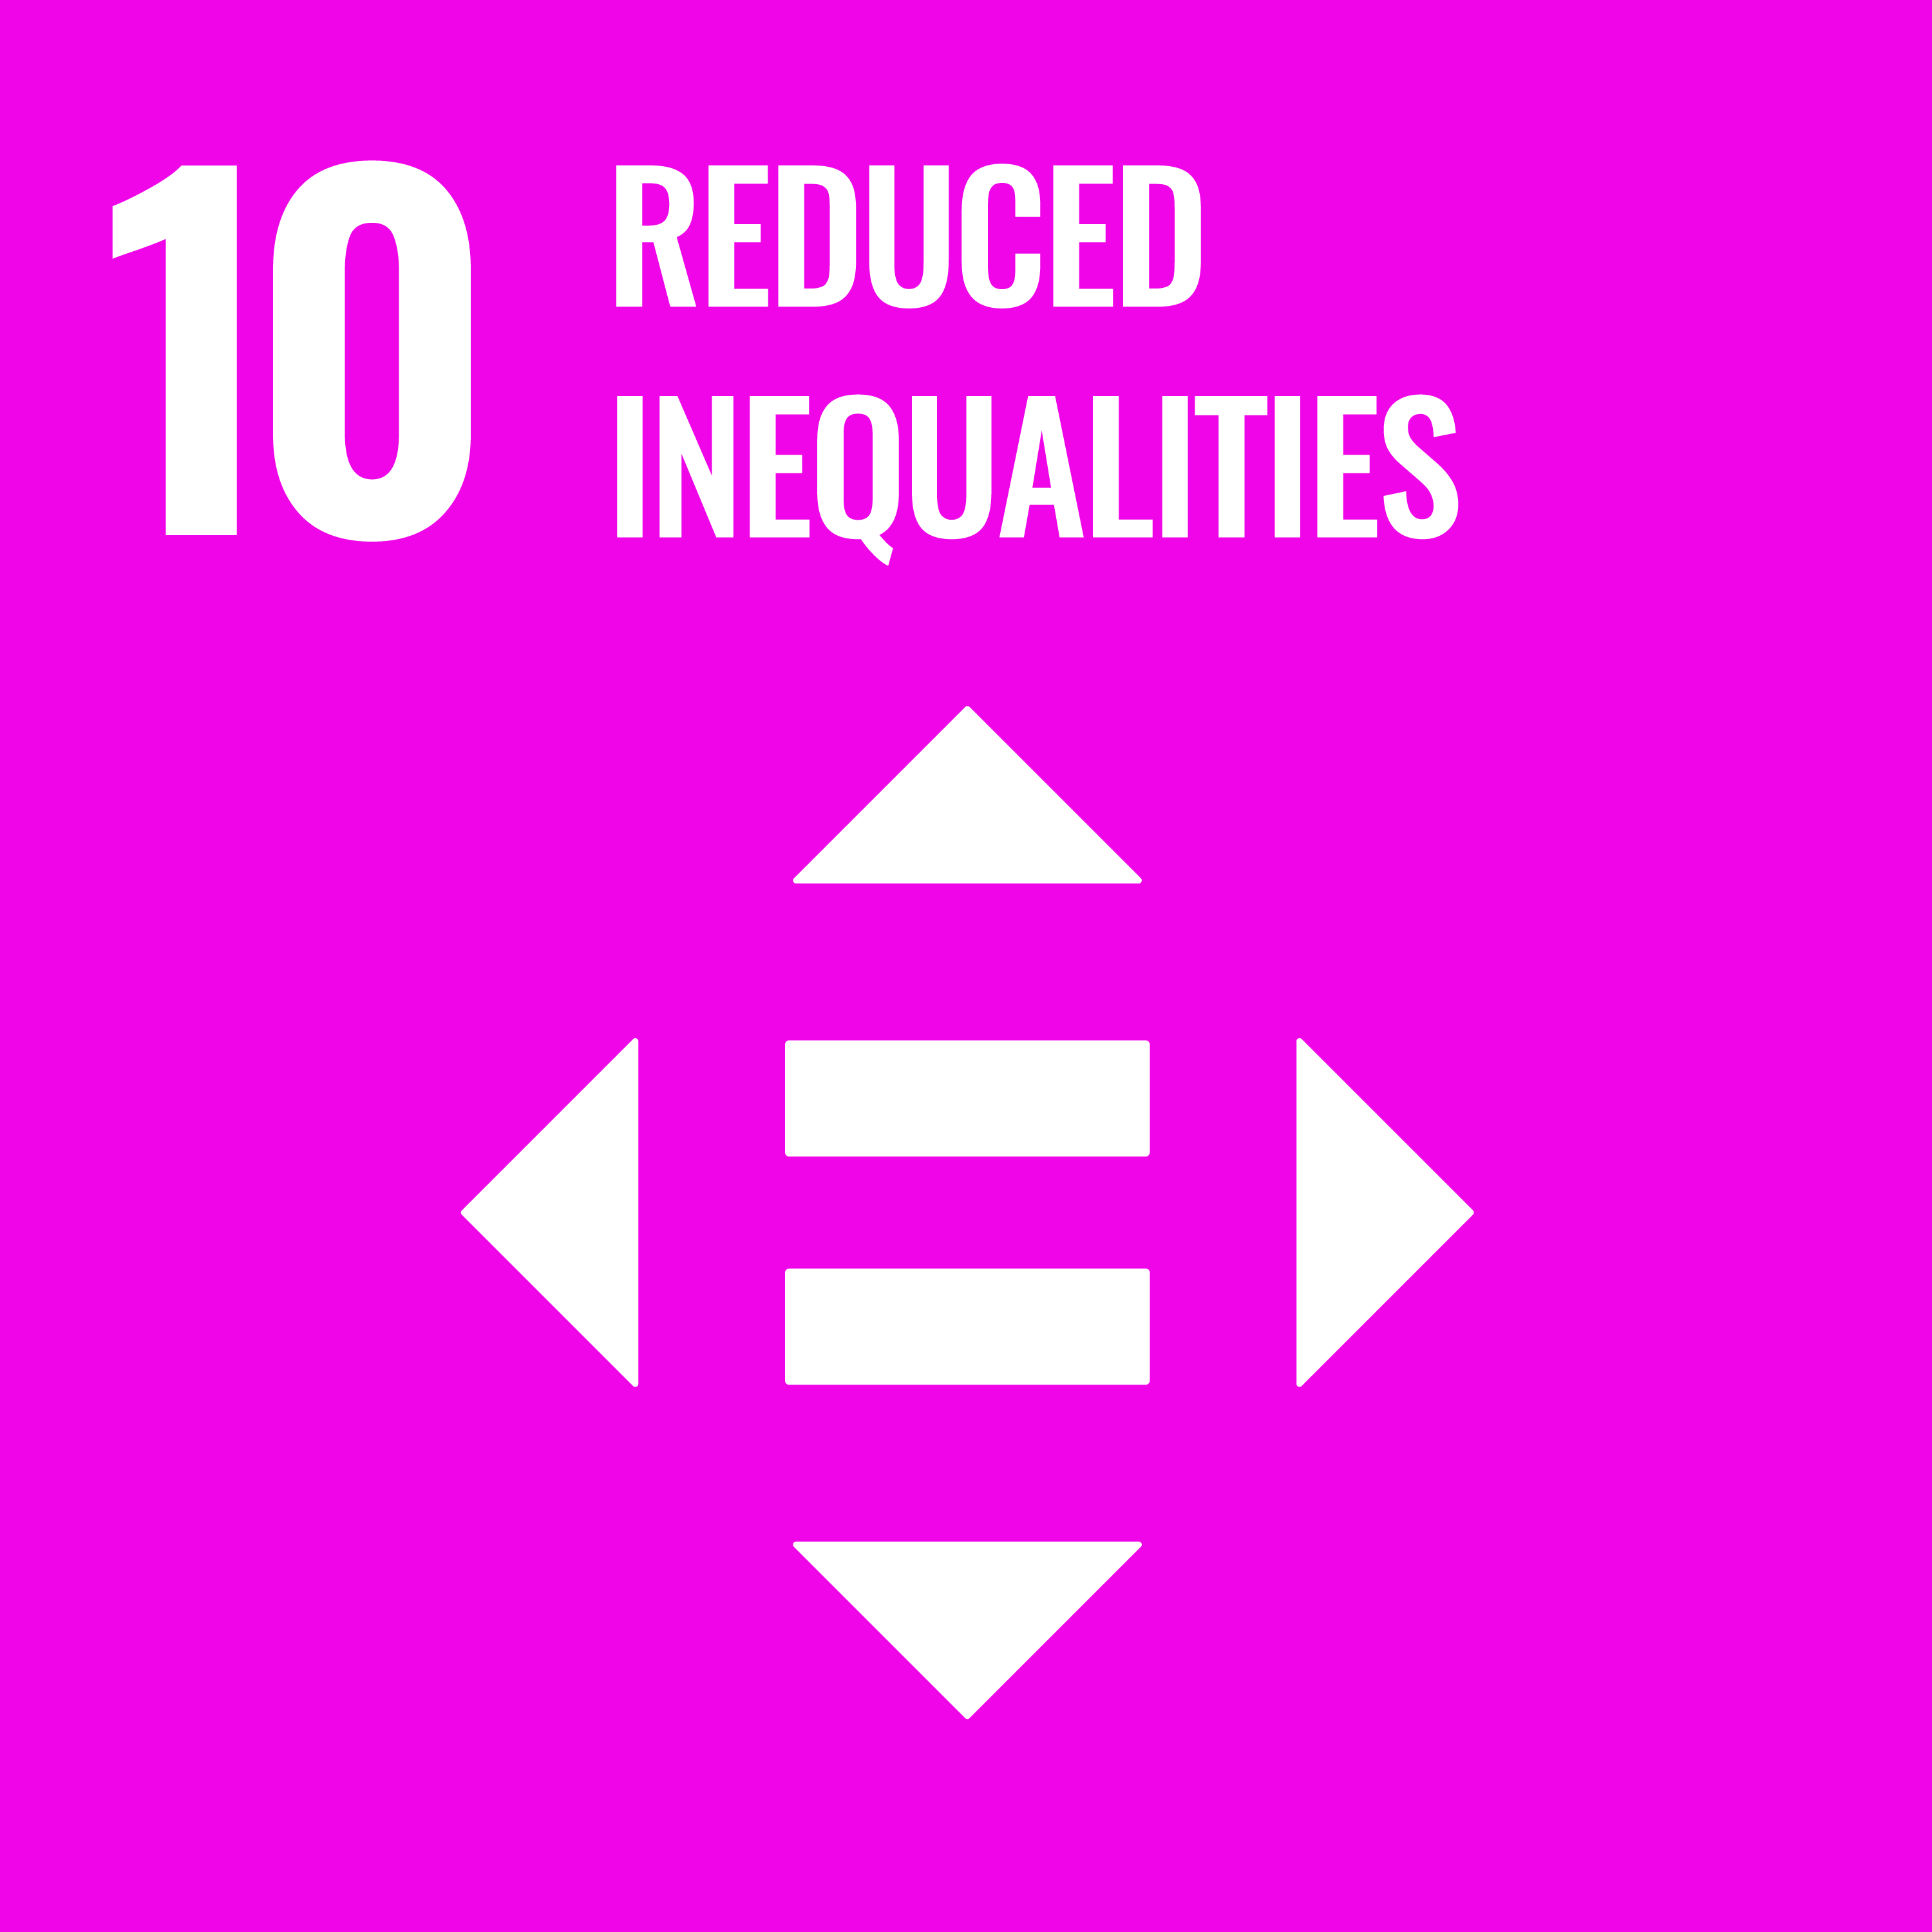
\includegraphics[width=0.25\linewidth]{Pictures/ODD/ODD10.jpg}%
	\hspace{0.5em}%
	\parbox[t]{0.7\linewidth}{\textbf{ODD 10 : Inégalités réduites} -- Réduire les inégalités dans les pays et d’un pays à l’autre.}
\end{minipage}

\vspace{1em}

\noindent
% Ligne 6
\begin{minipage}[t]{0.48\textwidth}
	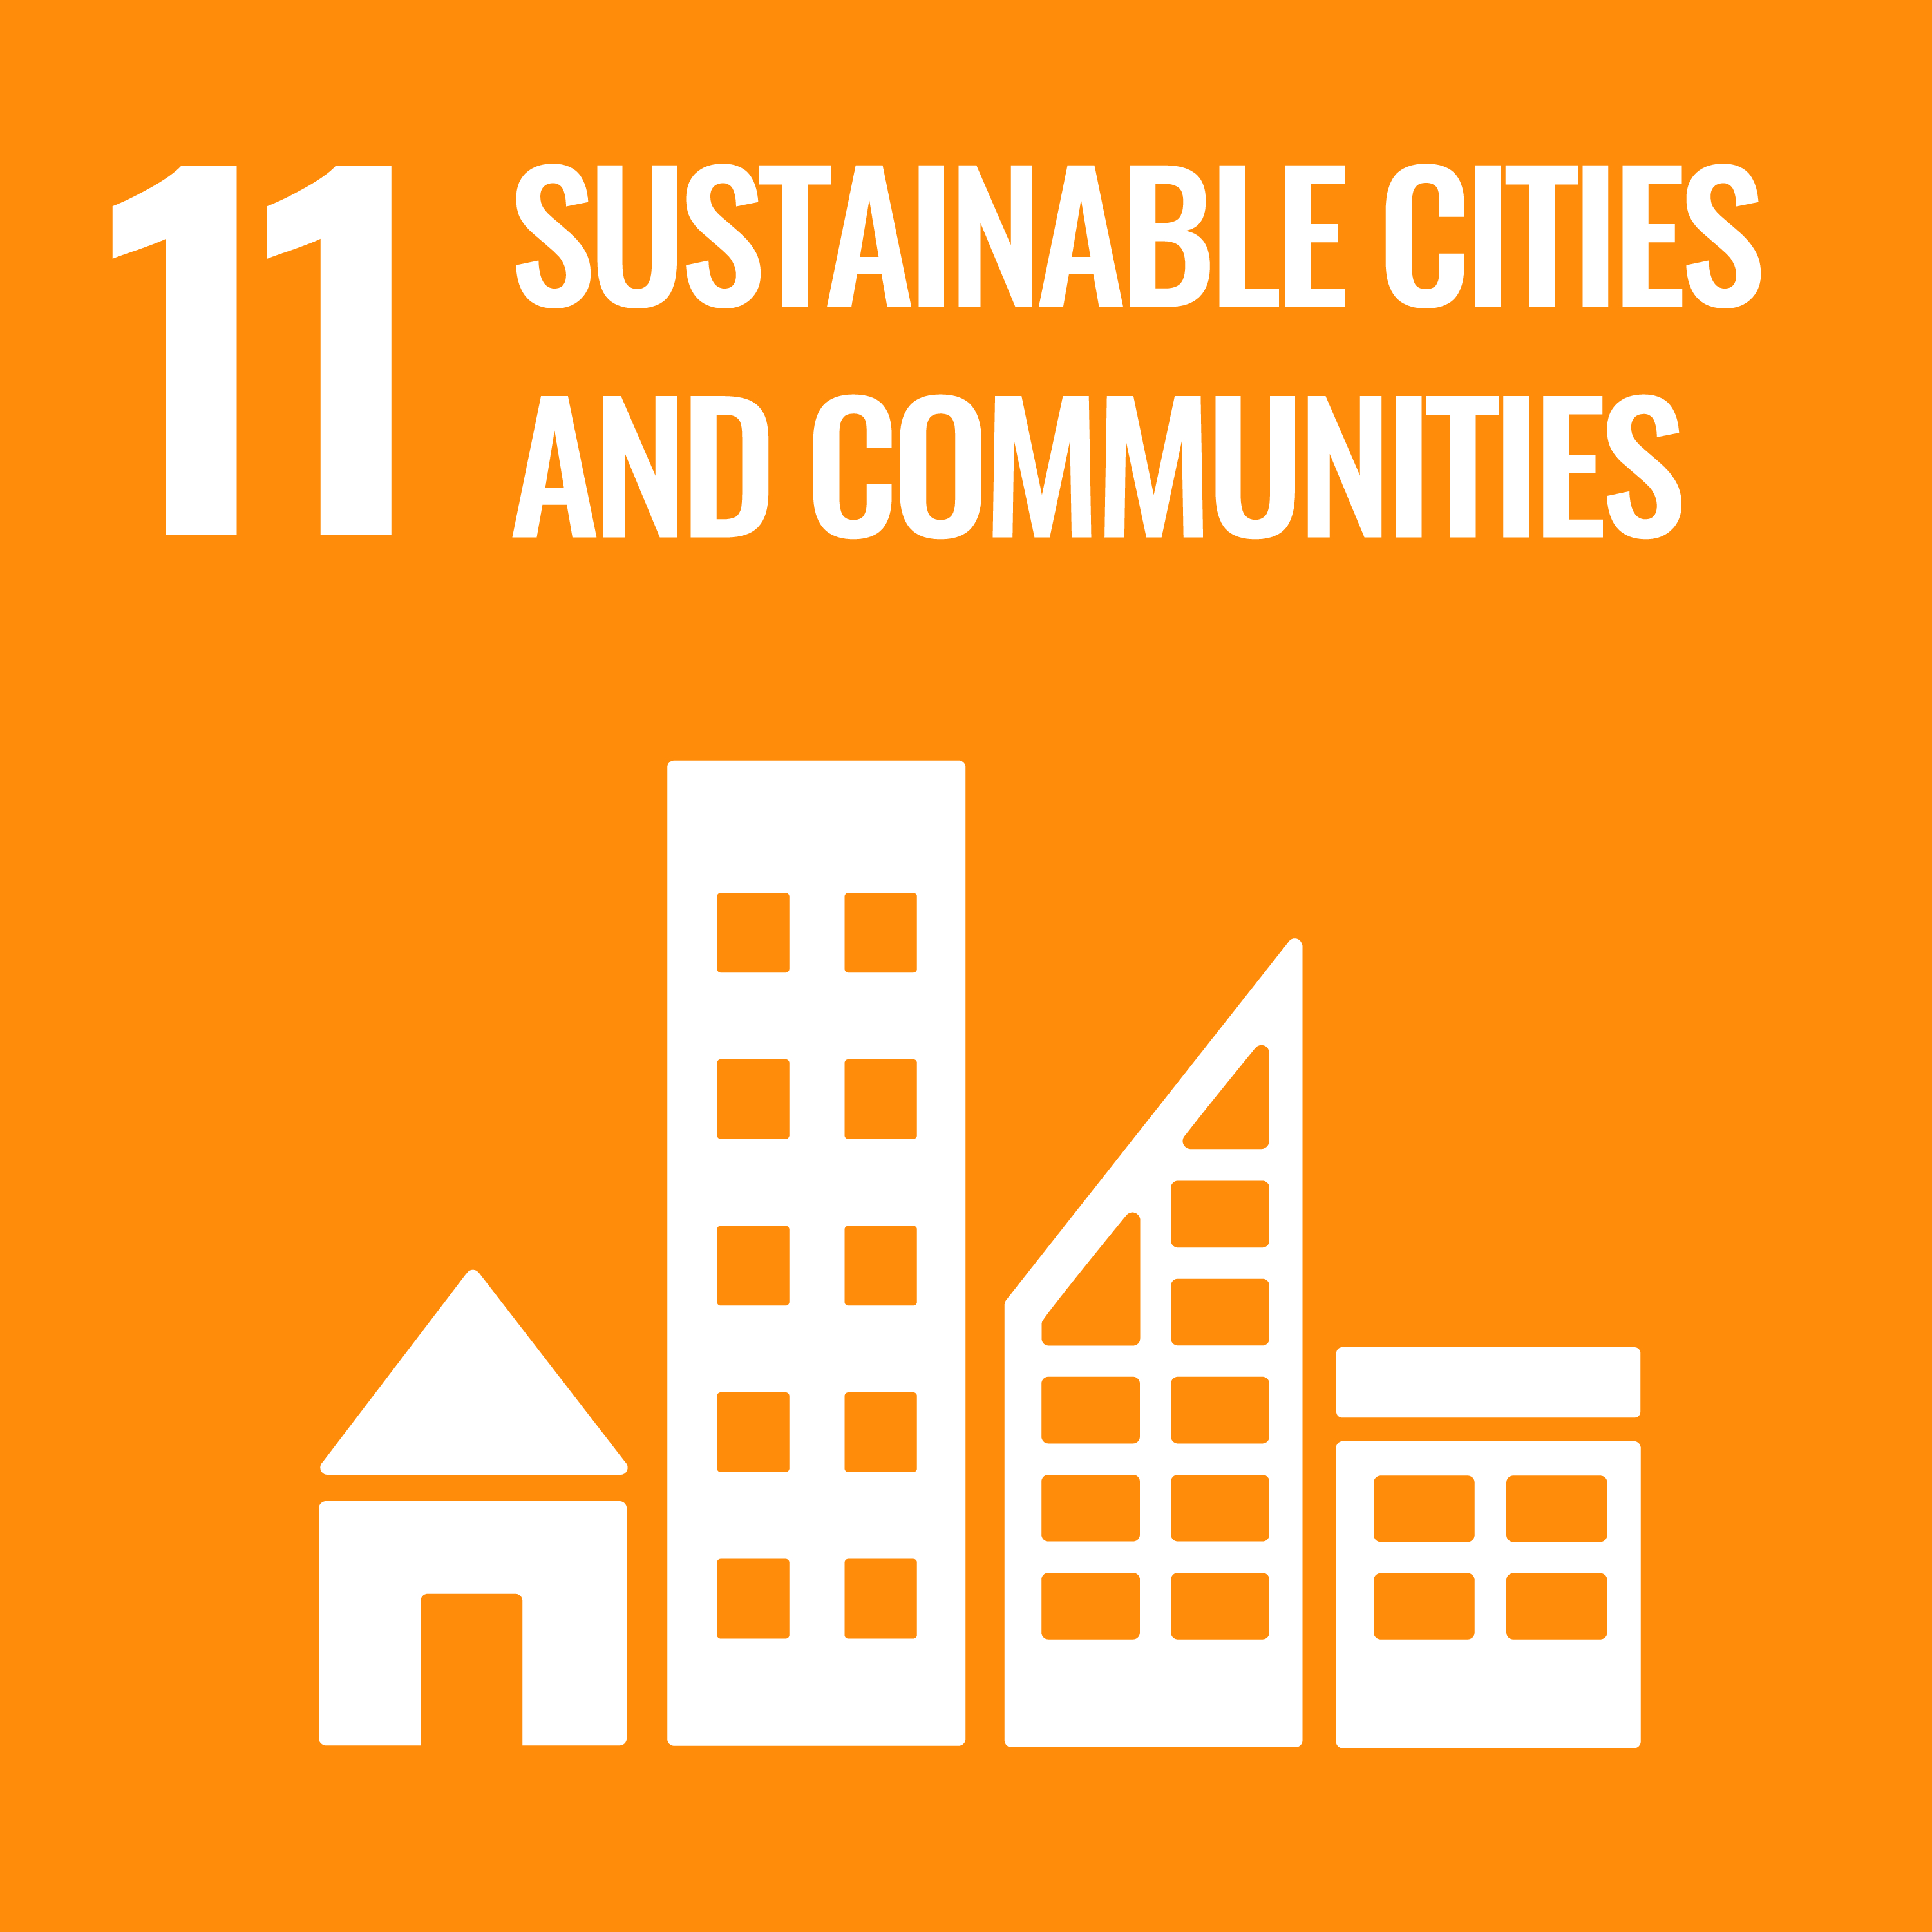
\includegraphics[width=0.25\linewidth]{Pictures/ODD/ODD11.jpg}%
	\hspace{0.5em}%
	\parbox[t]{0.7\linewidth}{\textbf{ODD 11 : Villes et communautés durables} -- Faire en sorte que les villes et les établissements humains soient ouverts à tous, sûrs, résilients et durables.}
\end{minipage}\hfill
\begin{minipage}[t]{0.48\textwidth}
	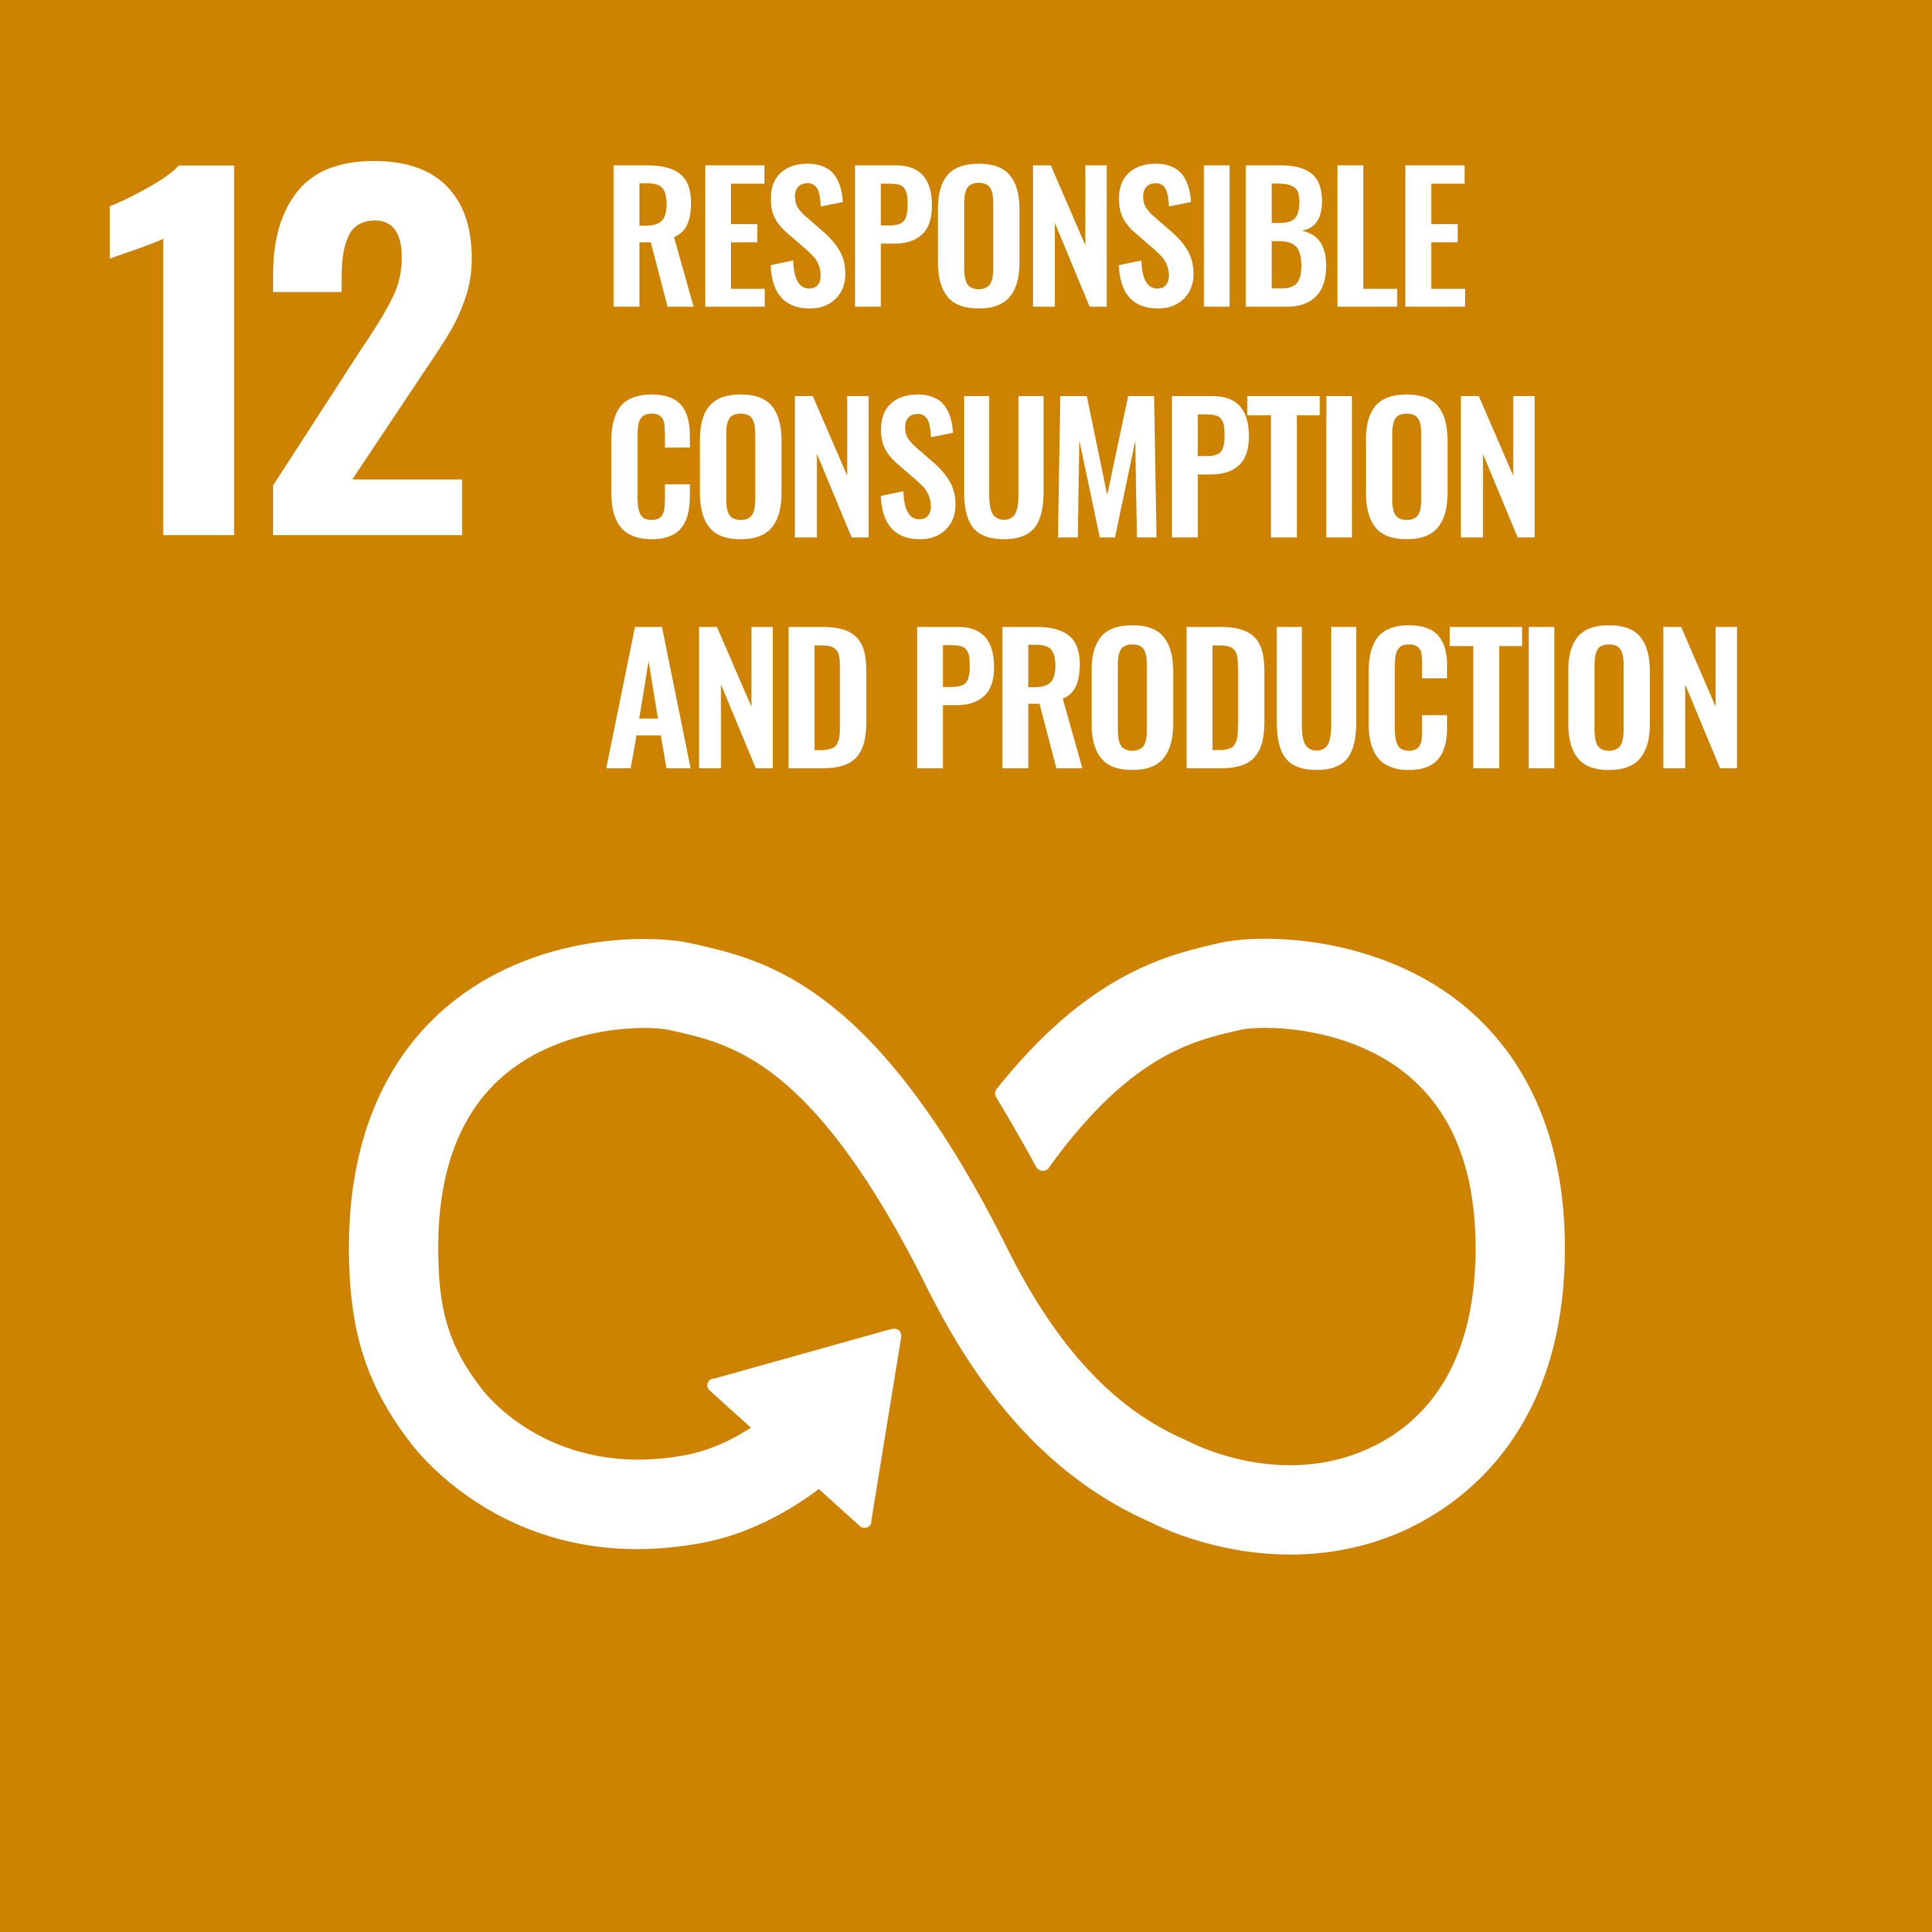
\includegraphics[width=0.25\linewidth]{Pictures/ODD/ODD12.jpg}%
	\hspace{0.5em}%
	\parbox[t]{0.7\linewidth}{\textbf{ODD 12 : Consommation et production responsables} -- Établir des modes de consommation et de production durables.}
\end{minipage}

\vspace{1em}

\noindent
% Ligne 7
\begin{minipage}[t]{0.48\textwidth}
	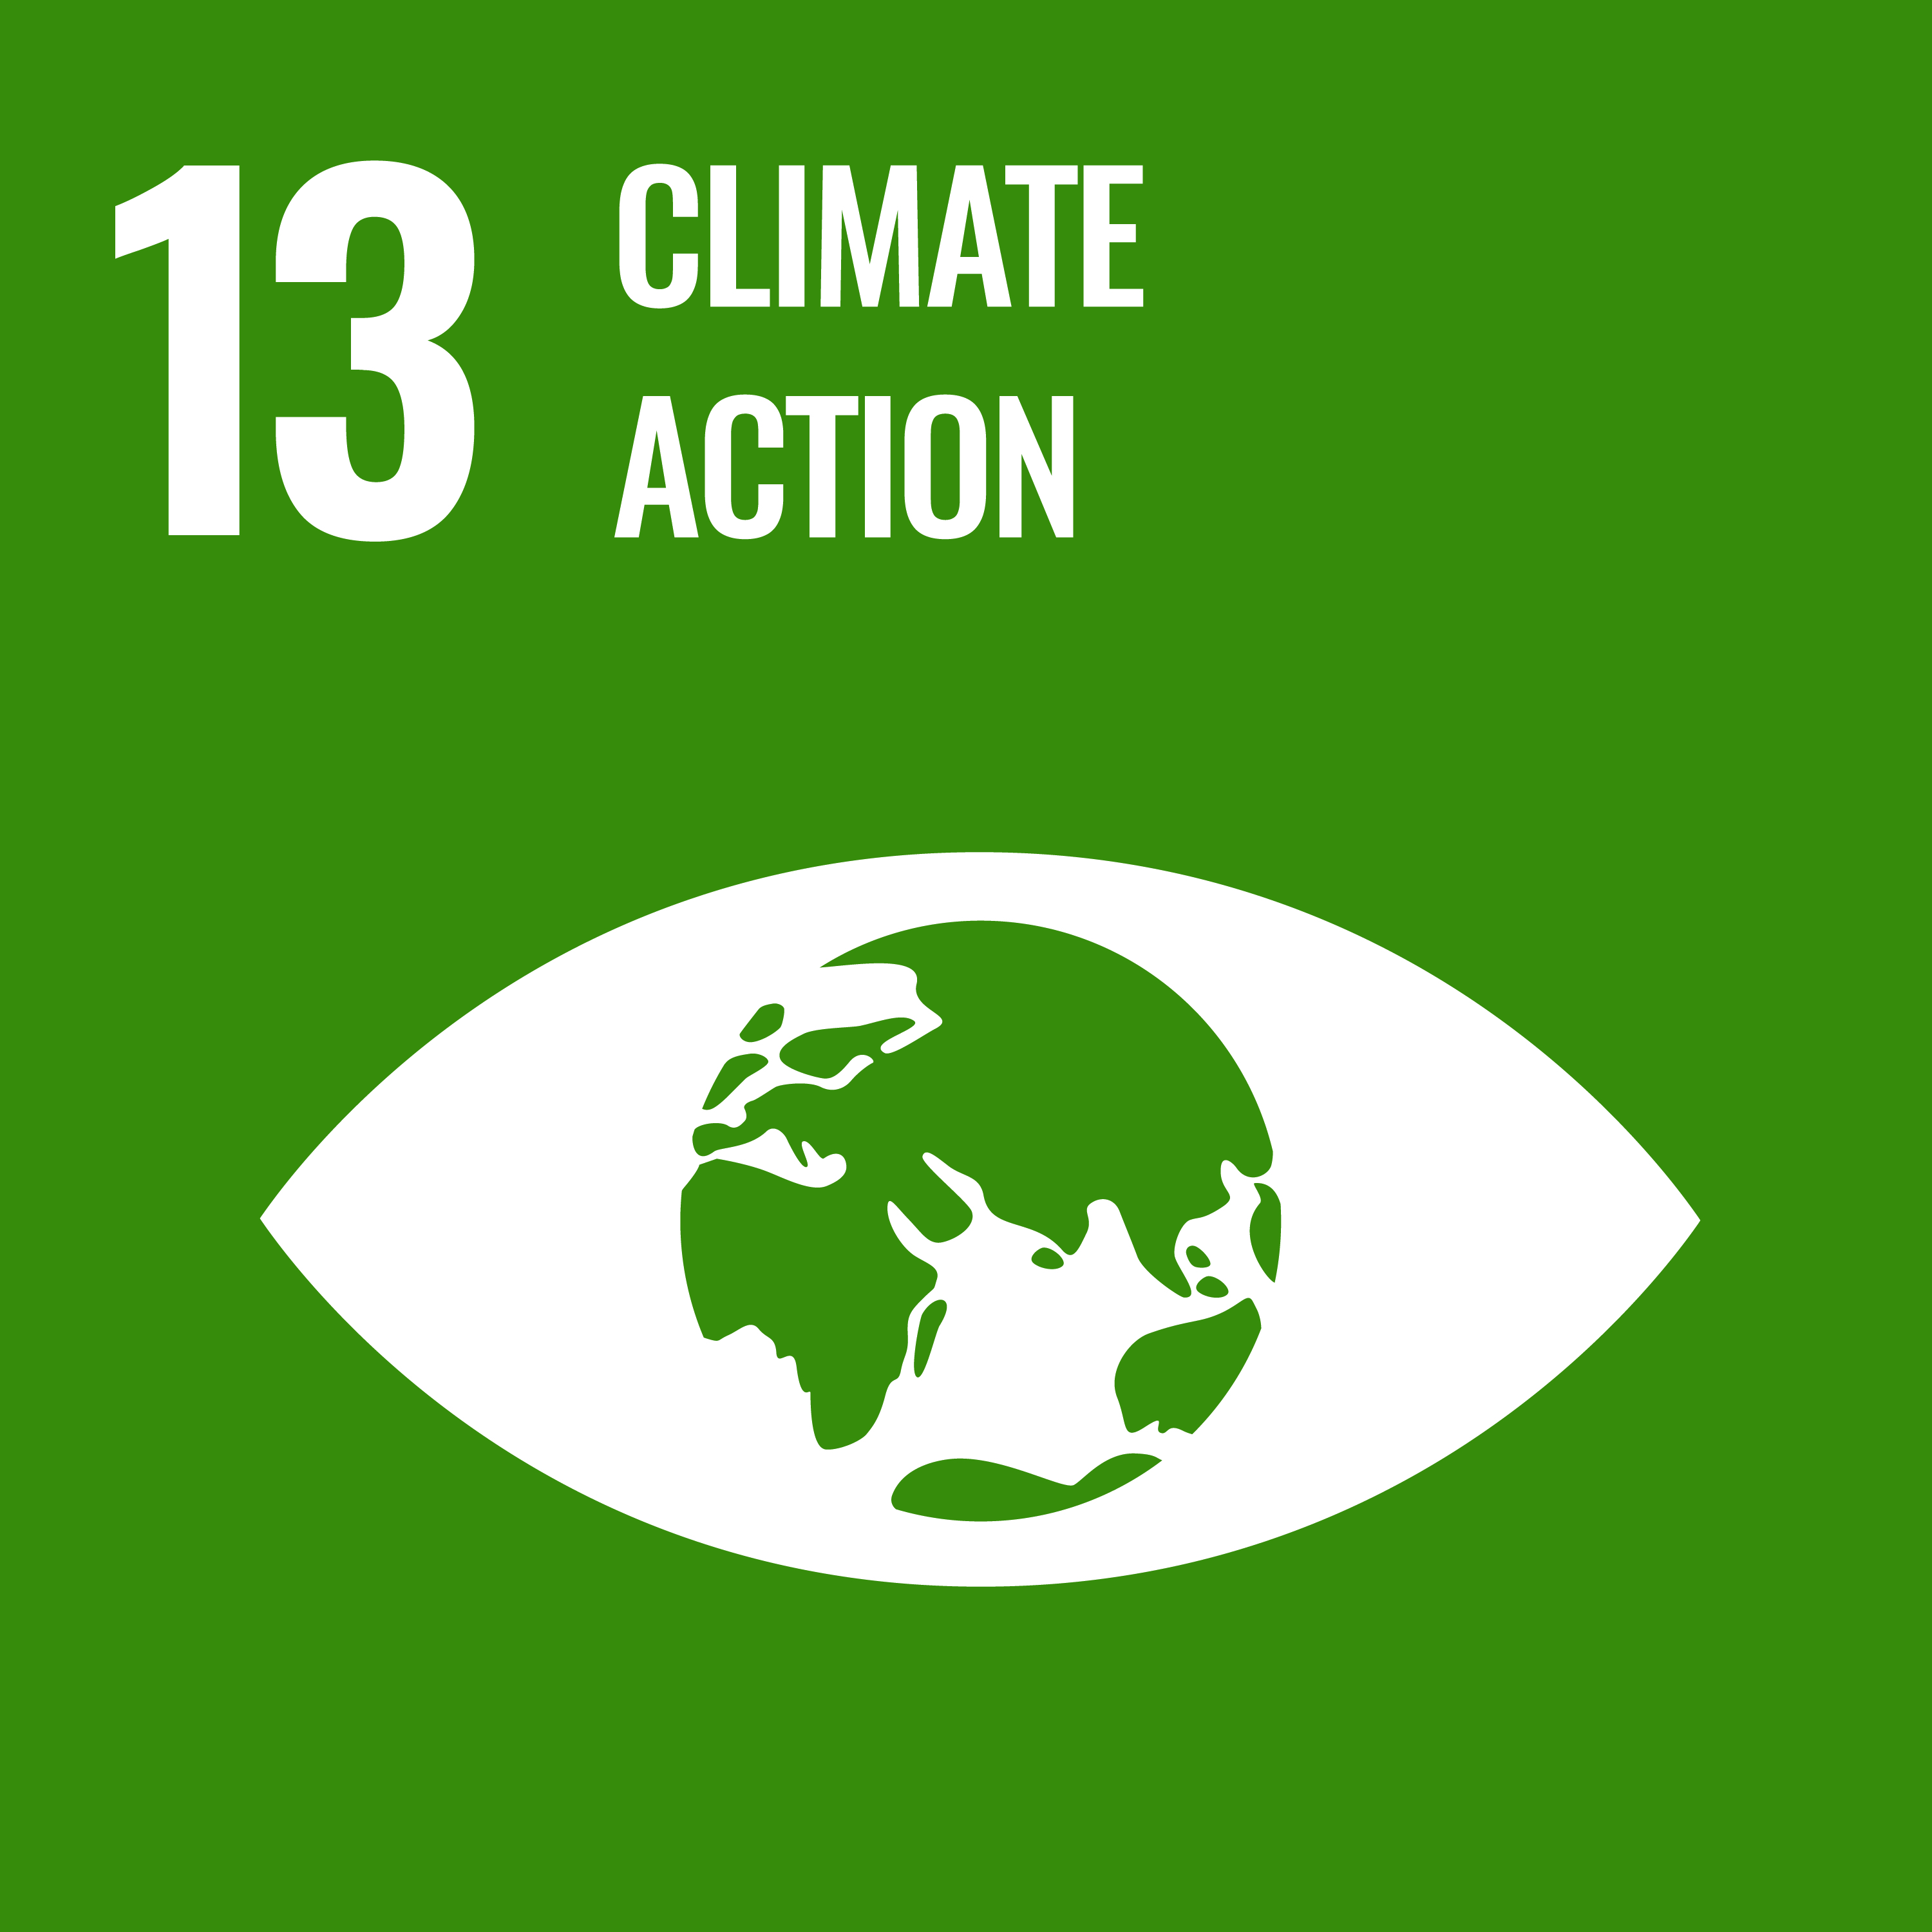
\includegraphics[width=0.25\linewidth]{Pictures/ODD/ODD13.jpg}%
	\hspace{0.5em}%
	\parbox[t]{0.7\linewidth}{\textbf{ODD 13 : Lutte contre les changements climatiques} -- Prendre d’urgence des mesures pour lutter contre les changements climatiques et leurs répercussions.}
\end{minipage}\hfill
\begin{minipage}[t]{0.48\textwidth}
	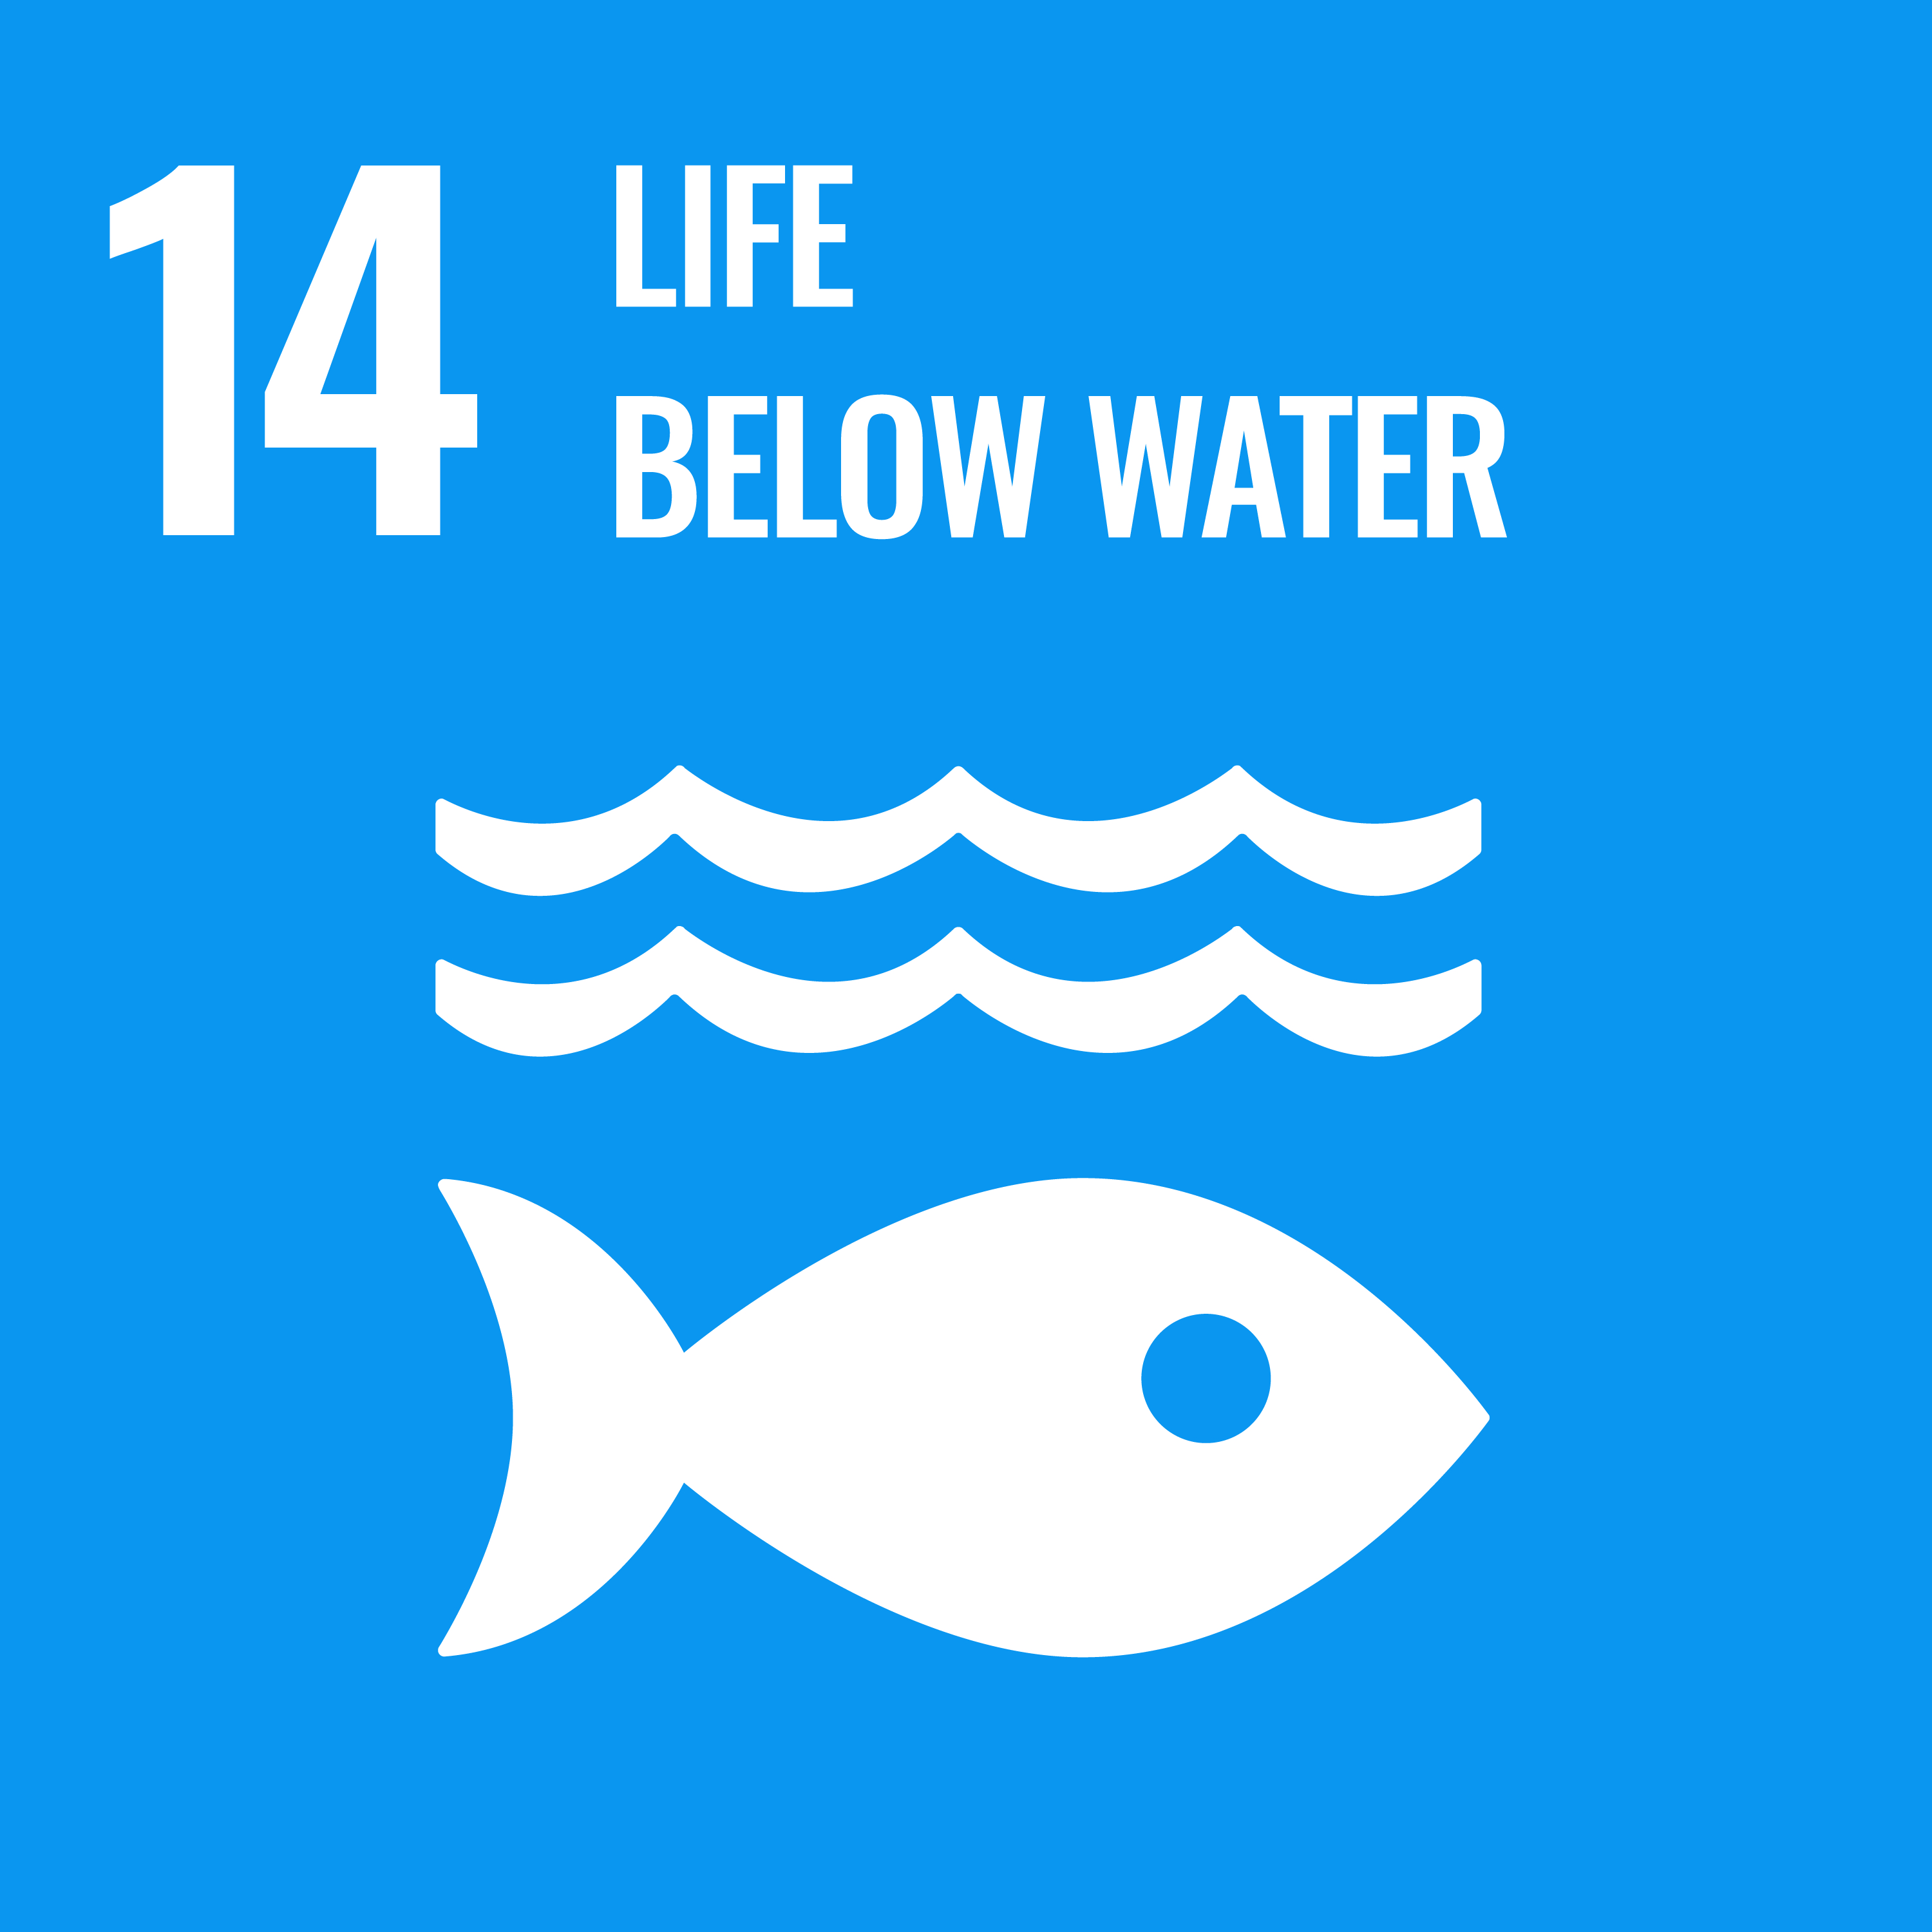
\includegraphics[width=0.25\linewidth]{Pictures/ODD/ODD14.jpg}%
	\hspace{0.5em}%
	\parbox[t]{0.7\linewidth}{\textbf{ODD 14 : Vie aquatique} -- Conserver et exploiter de manière durable les océans, les mers et les ressources marines aux fins du développement durable.}
\end{minipage}

\vspace{1em}

\noindent
% Ligne 8
\begin{minipage}[t]{0.48\textwidth}
	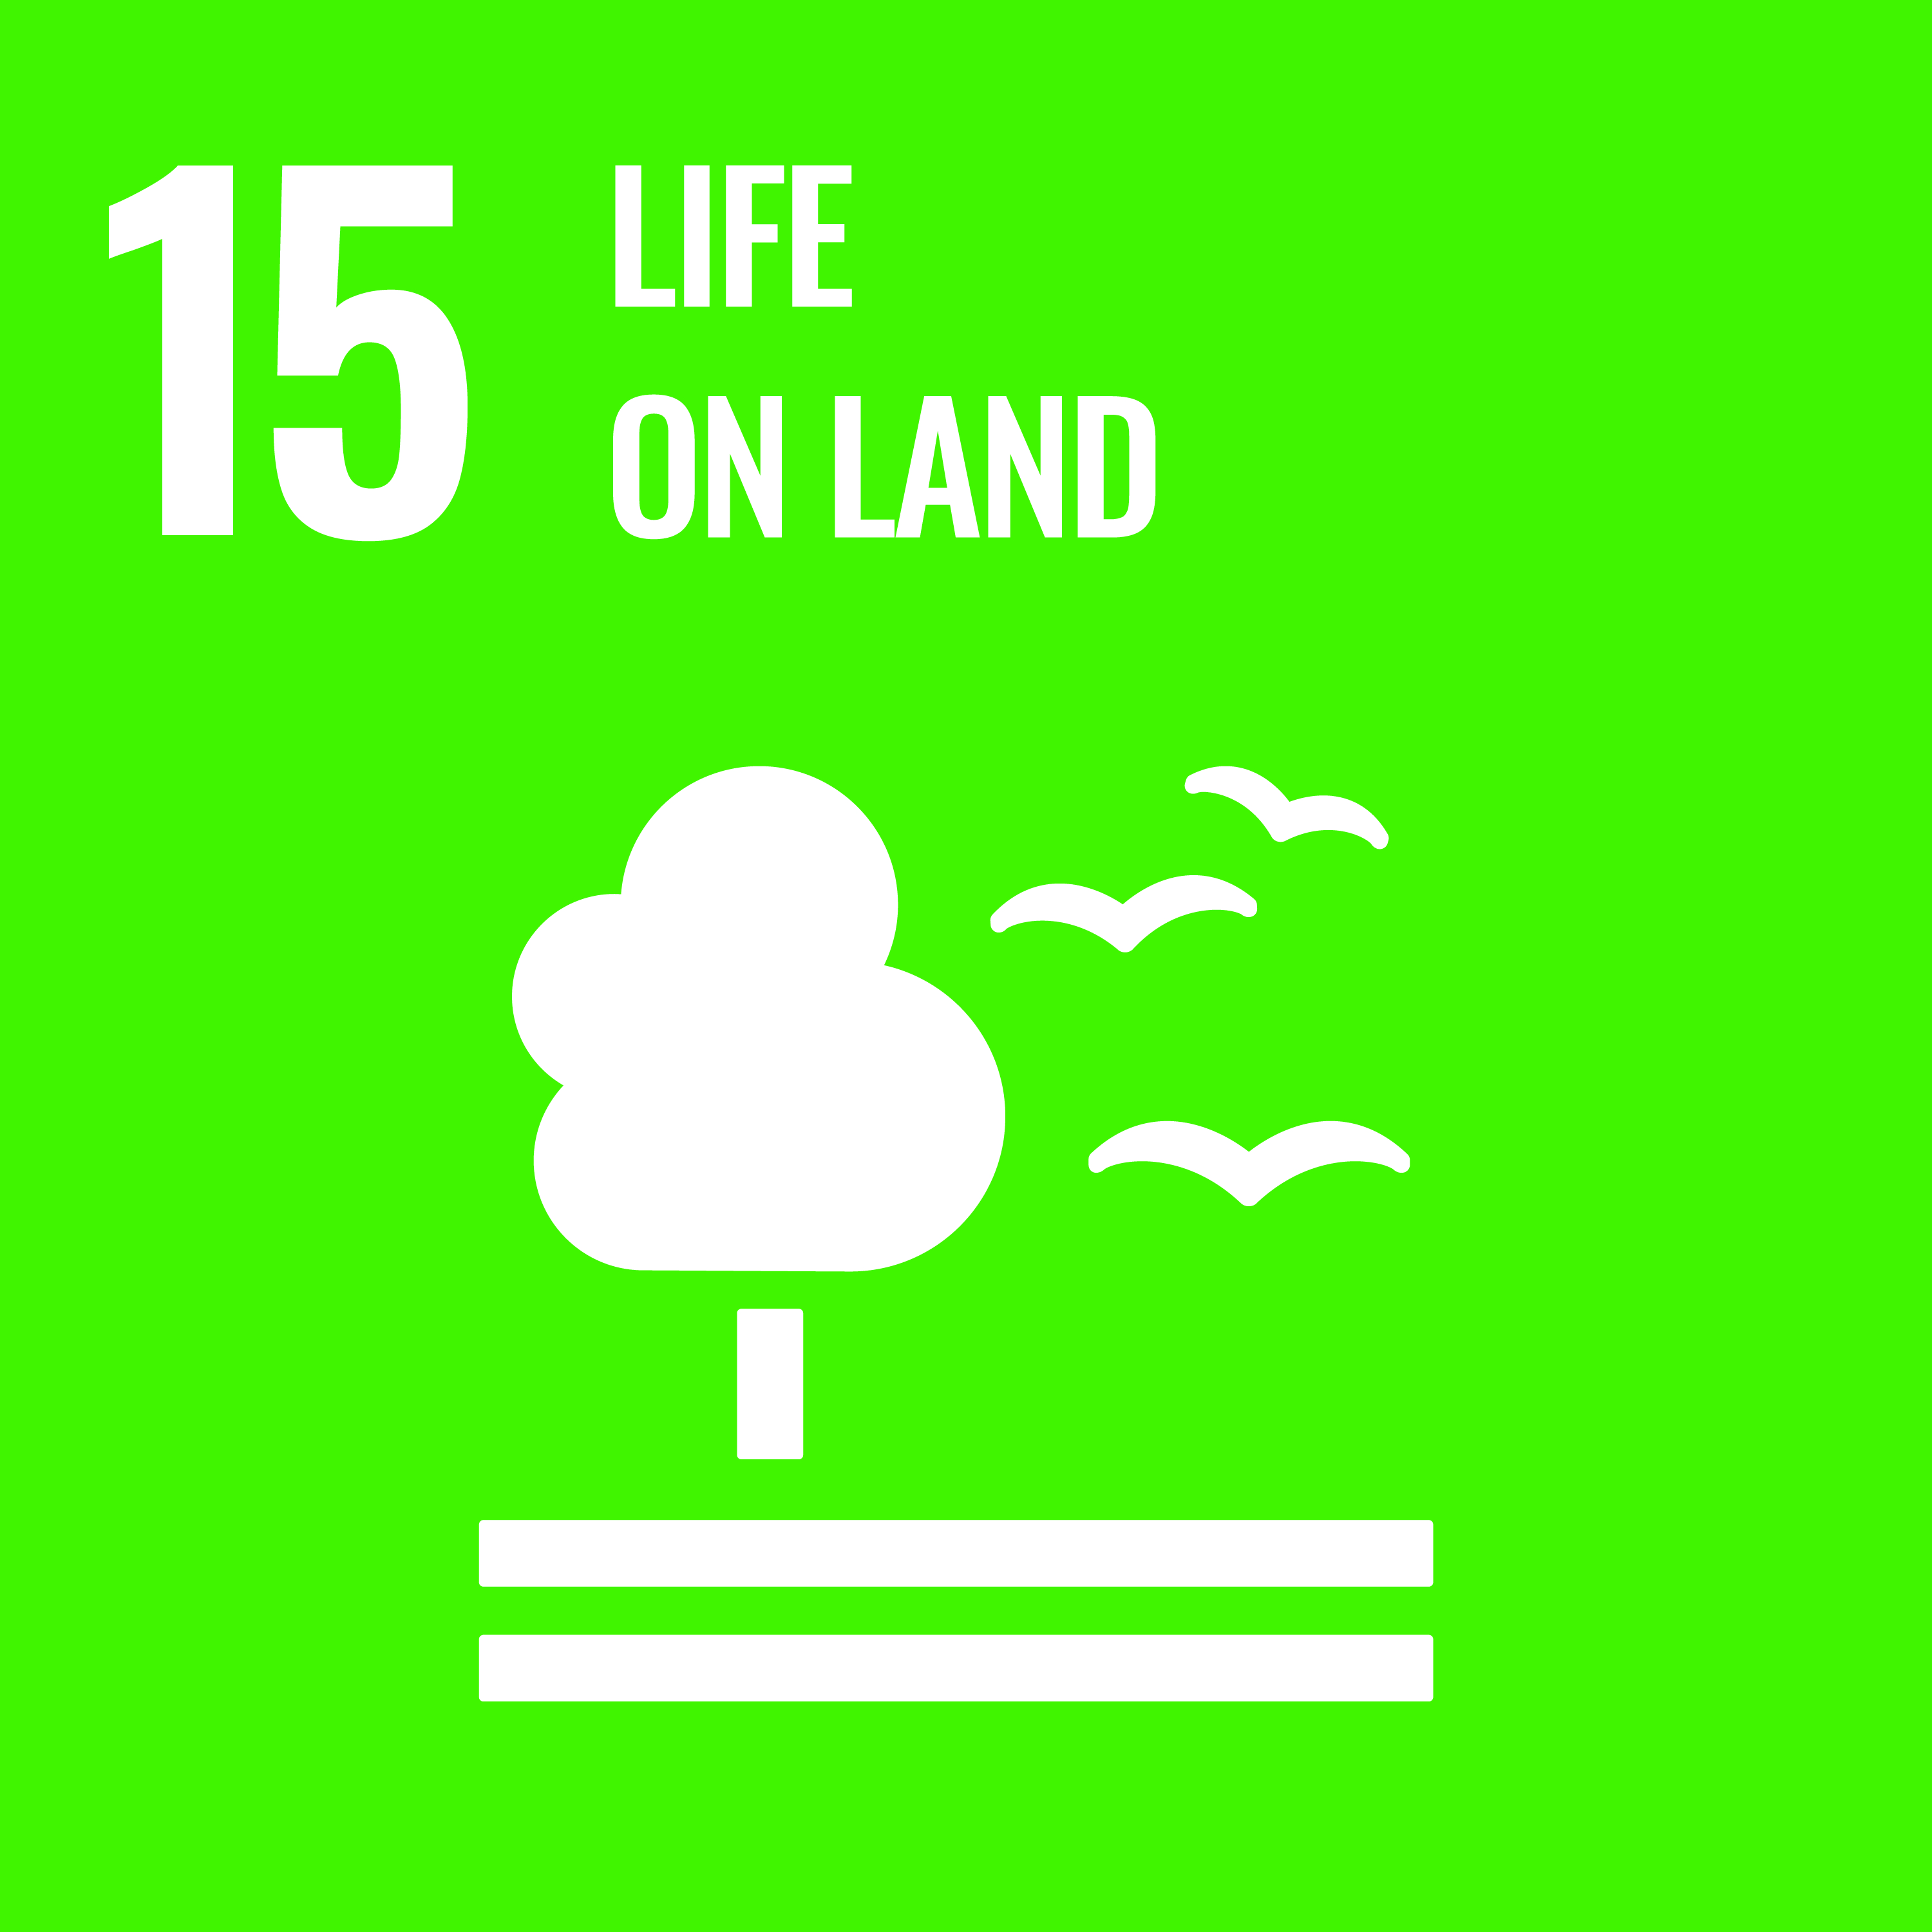
\includegraphics[width=0.25\linewidth]{Pictures/ODD/ODD15.jpg}%
	\hspace{0.5em}%
	\parbox[t]{0.7\linewidth}{\textbf{ODD 15 : Vie terrestre} -- Préserver et restaurer les écosystèmes terrestres, gérer durablement les forêts, lutter contre la désertification et mettre fin à l’appauvrissement de la biodiversité.}
\end{minipage}\hfill
\begin{minipage}[t]{0.48\textwidth}
	
\includegraphics[width=0.25\linewidth]{Pictures/ODD/ODD16.jpg}%
	\hspace{0.5em}%
	\parbox[t]{0.7\linewidth}{\textbf{ODD 16 : Paix, justice et institutions efficaces} -- Promouvoir l’avènement de sociétés pacifiques et inclusives, assurer l’accès de tous à la justice et mettre en place des institutions efficaces.}
\end{minipage}

\vspace{1em}

\noindent
% Ligne 9 (ODD 17 seul)
\begin{minipage}[t]{0.48\textwidth}
	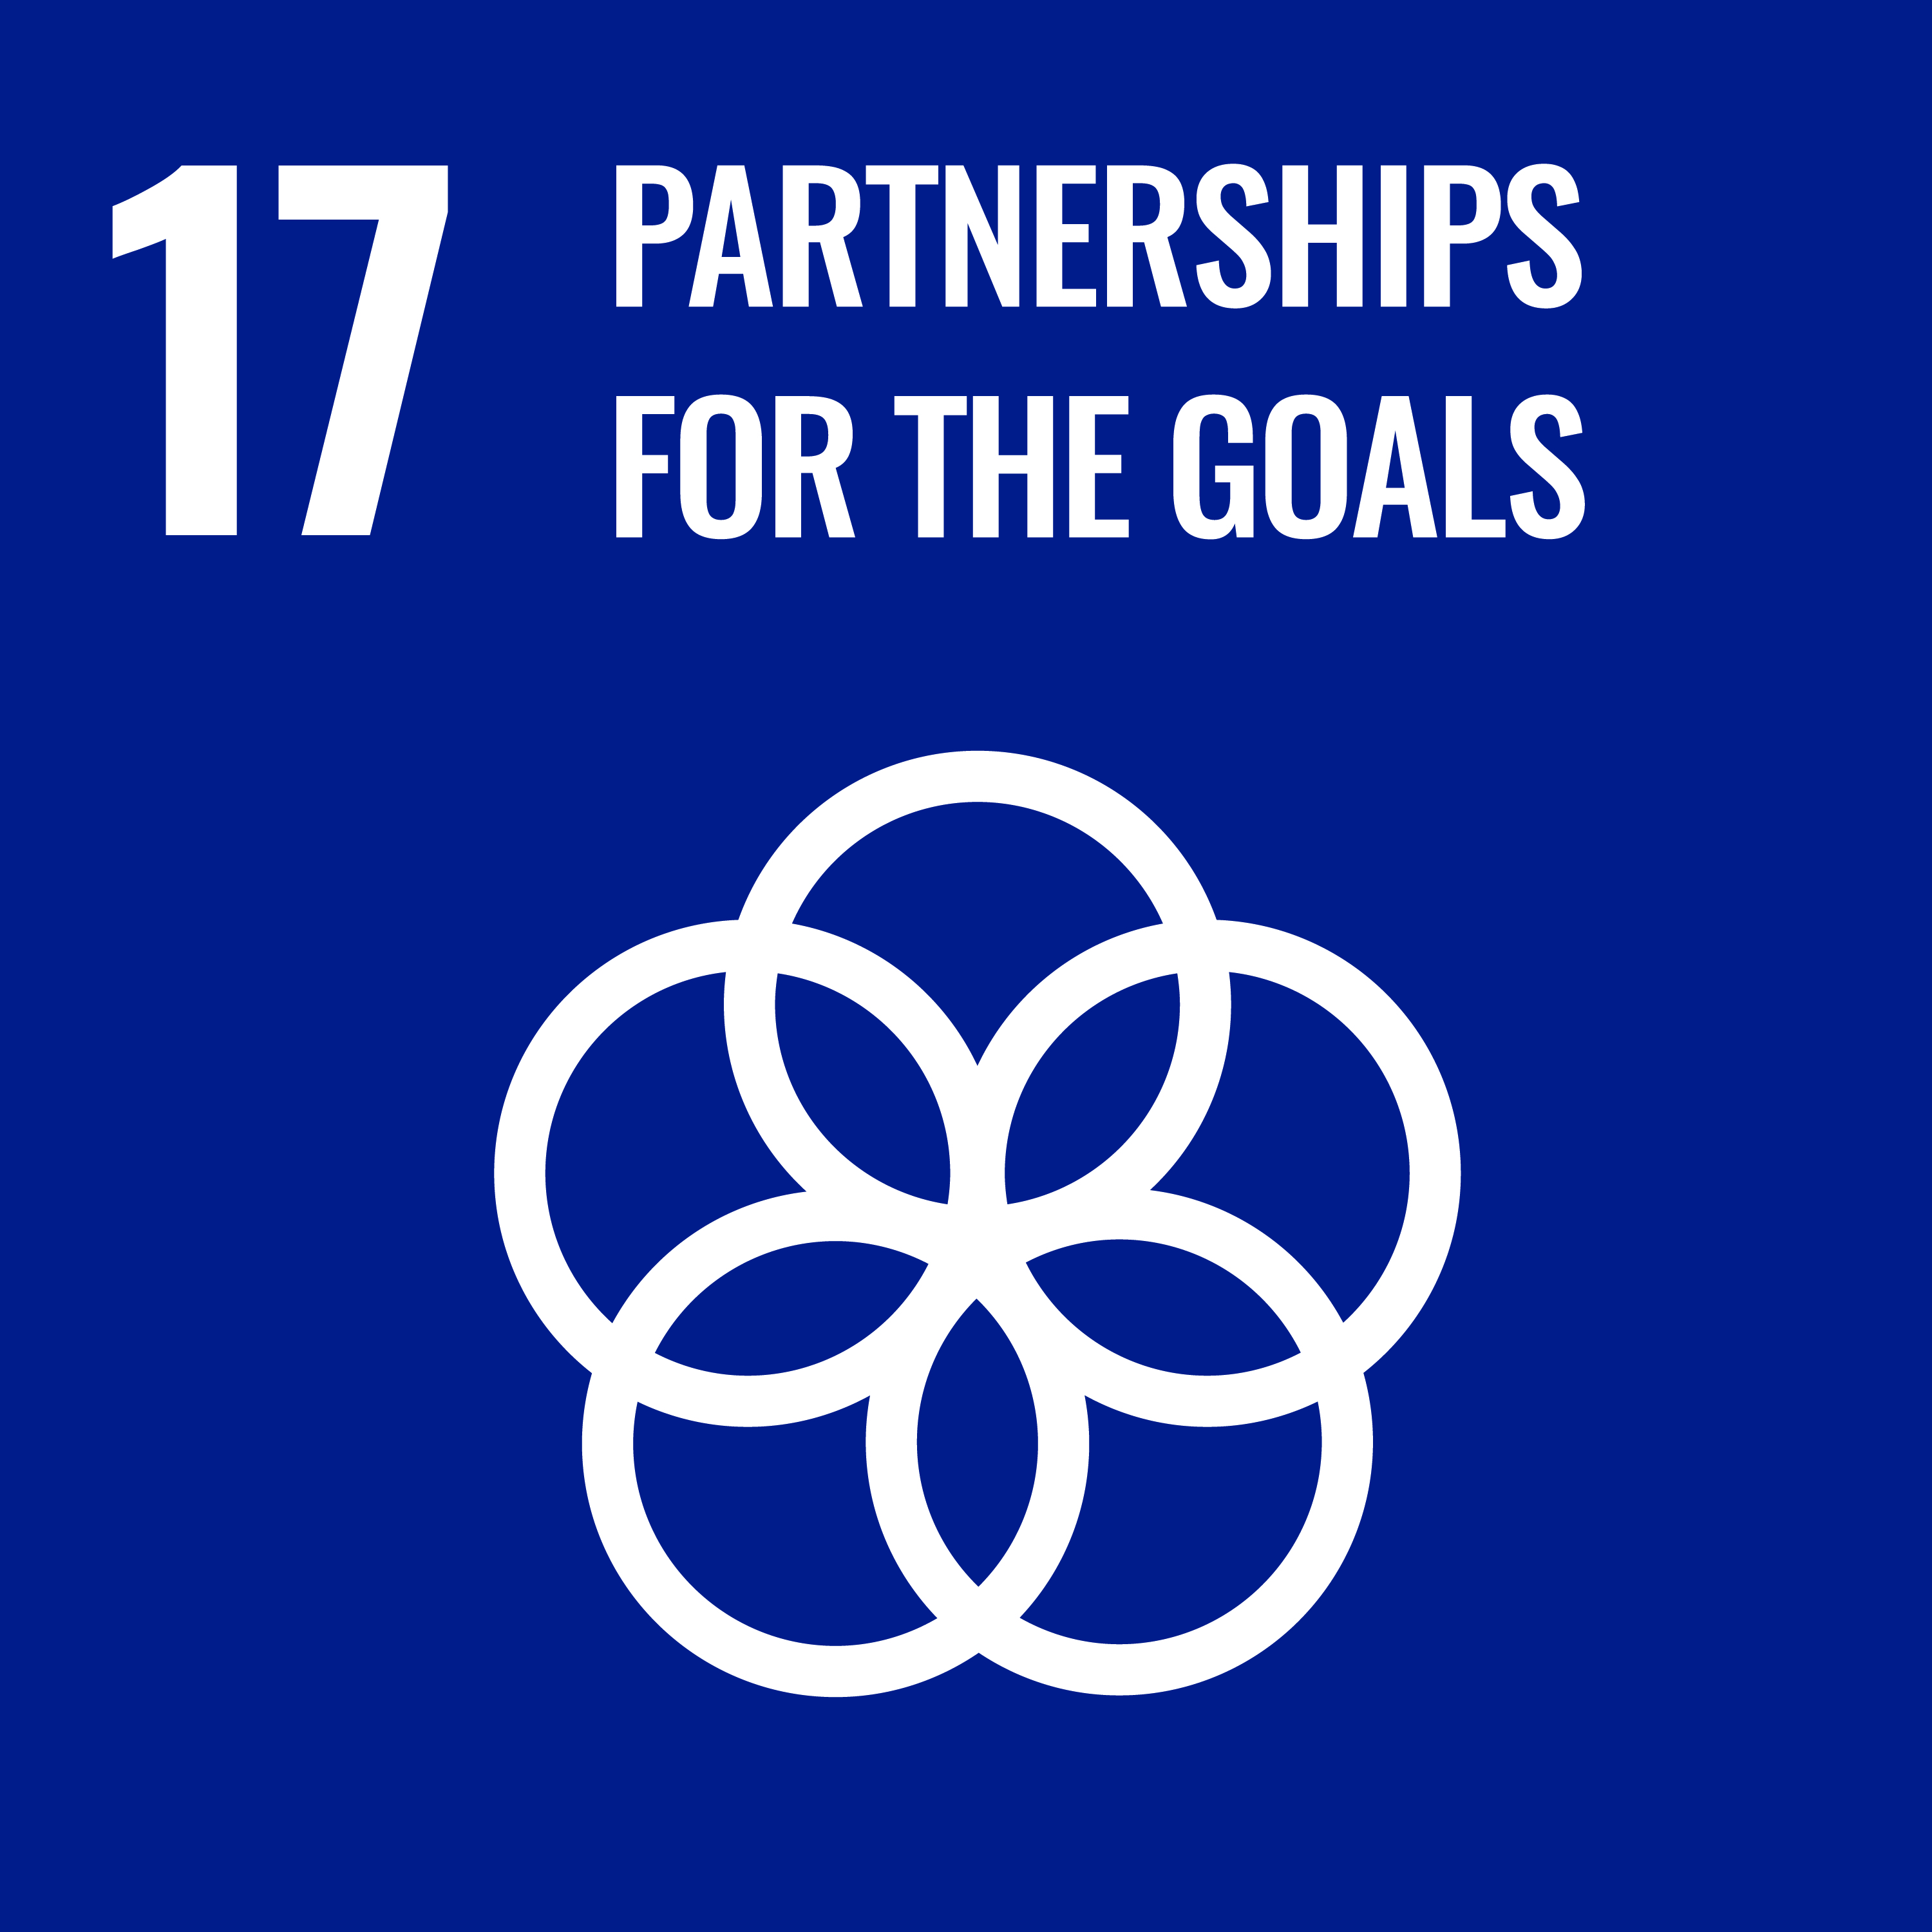
\includegraphics[width=0.25\linewidth]{Pictures/ODD/ODD17.jpg}%
	\hspace{0.5em}%
	\parbox[t]{0.7\linewidth}{\textbf{ODD 17 : Partenariats pour la réalisation des objectifs} -- Renforcer les moyens de mettre en œuvre le partenariat mondial pour le développement durable et le revitaliser.}
\end{minipage}








%===============================================














 
 
\subsection{Définitions des concepts clés}
\vspace{0.5cm}
\begin{simplebox}
\begin{enumerate}
	\item Un \textbf{indicateur} désigne une variable statistique, généralement quantitative, utilisée pour mesurer et suivre l’évolution d’un phénomène socio-économique ou environnemental. Dans le cadre des ODD, il permet d’évaluer de manière objective le degré de réalisation d’une cible donnée.
	
	\item Une \textbf{cible} correspond au niveau de résultat attendu pour un indicateur, tel que défini dans le cadre international des ODD ou dans une stratégie nationale. Elle constitue un seuil de référence permettant d’apprécier si les progrès réalisés sont conformes aux engagements pris.
	
	\item Un \textbf{indice composite} est une mesure synthétique obtenue par l’agrégation de plusieurs indicateurs élémentaires. Il vise à fournir une représentation globale d’un concept complexe – tel que le développement durable – qui ne peut être appréhendé par un seul indicateur.
\end{enumerate}
\end{simplebox}

 
 
%===============================================================


\subsection{Justification des indicateurs retenus}

Dans le cadre de ce rapport, certains indicateurs ont été retenus pour le calcul de l’ODD national, en tenant compte :  
\begin{itemize}
	\item de leur disponibilité statistique au niveau national ;
	\item de leur pertinence pour les priorités de développement du Sénégal ;
	\item de leur comparabilité avec les standards internationaux.
\end{itemize}

Lorsque les données nationales sont manquantes, des indicateurs alternatifs ou proxys sont utilisés afin d’assurer la continuité du suivi.








%========================= METHODOLOGIE ====================================








\section{Méthodologie de calcul de l'indicateur ODD}

Afin d'assurer la comparabilité entre les différents indicateurs, la valeur brute observée a été recalée sur une échelle de 0 à 100. Dans cette échelle normalisée, \textbf{0 représente la pire performance} possible et \textbf{100 correspond à la performance optimale (cible)}. Cette opération de normalisation est particulièrement sensible au choix des bornes utilisées, notamment la borne inférieure et la borne supérieure. Des valeurs extrêmes (outliers) peuvent en effet introduire des seuils involontaires et générer une variabilité artificielle dans les données.

La détermination des bornes repose sur un arbre décisionnel inspiré des standards internationaux de suivi des ODD :
\begin{simplebox}
\begin{enumerate}
	\item Lorsque l’ODD fournit un seuil quantitatif absolu (par exemple : zéro pauvreté, scolarisation universelle, égalité des sexes complète), celui-ci est utilisé comme \textbf{borne supérieure}.
	\item En l’absence de cible sexplicite, le principe du \textit{``Ne laisser personne de côté''} est appliqué, ce qui conduit à fixer la borne supérieure à une couverture universelle ou à une situation de zéro privation.
	\item Lorsqu’il existe des cibles scientifiques reconnues (par exemple, zéro émission nette de CO$_2$ d’ici 2050 ou gestion durable de 100\% des pêcheries), elles sont retenues comme borne supérieure.
	\item Pour les autres indicateurs, la borne supérieure est fixée à la \textbf{moyenne des cinq meilleurs performeurs mondiaux}.
\end{enumerate}
\end{simplebox}


La \textbf{borne inférieure}, quant à elle, est définie par le \textbf{2,5\textsuperscript{e} percentile de la distribution internationale} de l’indicateur, conformément aux bonnes pratiques statistiques de mesure de la performance relative.

Le calcul de l’indice normalisé s’effectue selon la formule suivante :

\begin{simplebox2}

\[
x' = \frac{x - \text{min}}{\text{max} - \text{min}} \times 100
\]
\end{simplebox2}

où $x$ désigne la valeur brute observée, $\text{min}$ la borne inférieure, $\text{max}$ la borne supérieure, et $x'$ la valeur normalisée sur l’échelle 0--100.

Ainsi, un pays obtenant un score de 50 est situé à mi-chemin entre la performance minimale et l’optimum, tandis qu’un score de 75 traduit une couverture de trois quarts de la distance vers la cible.

